\documentclass[xcolor=table]{beamer}
\usetheme{uic}
\usepackage{minted}
\usepackage{amsfonts,amsmath,oldgerm,algorithmic,algorithm}
\usepackage[font=small,labelfont=bf]{caption} % Required for specifying captions to tables and figures
\usepackage{tcolorbox}
\tcbuselibrary{listings,skins}
\usepackage{alltt,xcolor}
\usepackage{hyperref}
\usepackage{comment}
\usepackage{amsthm}
\usepackage{breqn}

\usepackage[spanish]{babel}


\lstdefinestyle{mystyle}{
language=C
}

\newtcblisting{mylisting}[2][]{
    arc=0pt, outer arc=0pt,
    listing only, 
    listing style=mystyle,
    title=#2,
    #1
}


\newcommand{\hrefcol}[2]{\textcolor{uihteal}{\href{#1}{#2}}}
\newcommand{\testcolor}[1]{\colorbox{#1}{\textcolor{#1}{test}}~\texttt{#1}}

% Please see Section 18.1 of Beamer User Guide for all the options \usefonttheme provides
\usefonttheme[onlymath]{serif}
% \usefonttheme{serif} % use this if you would like Serif font throughout (and not just for math)

\title{Fundamentos de Inteligencia Artificial}
\titlebackground{images/etsiinformatica3.jpeg}
% an asterisk will split the background:
% \titlebackground*{images/uic_seo.jpg}
\subtitle{Complejidad de algoritmos y calculabilidad de problemas}

\author{\href{mailto:jmmontes@uma.es}{José A. Montenegro}}
\date{\today}



\begin{document}

\newtheorem{mydef}{Definición}[section] % Añade [section] para que se reinicie en cada sección
\maketitle

% default is no footline, but page numbers are incredibly useful for the audience to ask questions later
\footlinecolor{uicblue}

%%%%%%%%%%%%%%%%%%%%%%%%%%%%%%%%%%%%%%%%%%%%%%%%%%%
%%%%%%%%%%%%%%%%%%%%%%%%%%%%%%%%%%%%%%%%%%%%%%%%%%%
%%%%%%%%%%%%%%%%%%%%%%%%%%%%%%%%%%%%%%%%%%%%%%%%%%%
%%%%%%%%%%%%%%%%%%%%%%%%%%%%%%%%%%%%%%%%%%%%%%%%%%%
%%%%%%%%%%%%%%%%%%%%%%%%%%%%%%%%%%%%%%%%%%%%%%%%%%%
%%%%%%%%%%%%%%%%%%%%%%%%%%%%%%%%%%%%%%%%%%%%%%%%%%%


%%%%%%%%%%%%%%%%%%%%%%%%%%%%%%%%%%%%%%%%%%%%%%%%%%%
%%%%%%%%%%%%%%%%%%%%%%%%%%%%%%%%%%%%%%%%%%%%%%%%%%%
%%%%%%%%%%%%%%%%%%%%%%%%%%%%%%%%%%%%%%%%%%%%%%%%%%%
%%%%%%%%%%%%%%%%%%%%%%%%%%%%%%%%%%%%%%%%%%%%%%%%%%%
%%%%%%%%%%%%%%%%%%%%%%%%%%%%%%%%%%%%%%%%%%%%%%%%%%%
%%%%%%%%%%%%%%%%%%%%%%%%%%%%%%%%%%%%%%%%%%%%%%%%%%%


\begin{frame}{Contenido}
\tableofcontents
\end{frame}


%%%%%%%%%%%%%%%%%%%%%%%%%%%%%%%%%%%%%%%%%%%%%%%%%%%
%%%%%%%%%%%%%%%%%%%%%%%%%%%%%%%%%%%%%%%%%%%%%%%%%%%
%%%%%%%%%%%%%%%%%%%%%%%%%%%%%%%%%%%%%%%%%%%%%%%%%%%

\begin{chapter}[images/etsiinformatica4.png]{uicblue}{Formalización del concepto de algoritmo}
\end{chapter}

\section{Formalización del concepto de algoritmo}


%%%%%%%%%%%%%%%%%%%%%%%%%%%%%%%%
\begin{frame}[fragile]\frametitle{Formalización del concepto de algoritmo} \scriptsize


\begin{columns}
\begin{column}{0.15\textwidth}

\begin{center}

\includegraphics[width=\textwidth]{images/Al-Khwarizmi_portrait.jpg}    
\end{center}

\end{column}

\begin{column}{0.75\textwidth}

En el siglo VIII, el califa de Bagdad Hârûn al-Rasîd fundó “La casa de la Sabiduría”, impulsada luego por su hijo el califa al-Ma'mûn (786-833), como un lugar para el desarrollo y protección del saber y los sabios. \\

\textit{Abu Ja'far Mohammed ibn Musa al-Khowârizmî} (780-850) fue miembro de la casa de la sabiduría, de su nombre procede la palabra \textbf{algoritmo} cuya forma original era \textbf{algorismo}.\\

\end{column}
\end{columns}


\begin{columns}
\begin{column}{0.15\textwidth}

\begin{center}
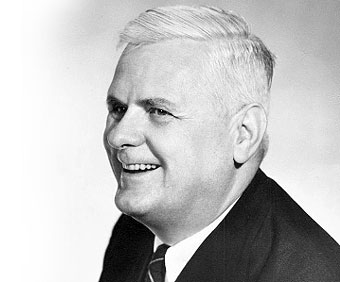
\includegraphics[width=\textwidth]{images/church_alonzo.jpg}    
\end{center}

\end{column}

\begin{column}{0.75\textwidth}


En abril de 1935, \textit{Alonzo Church} presentó una comunicación donde formalizaba las funciones recursivas en términos del \textbf{$\lambda$-cálculo} y enunció la equivalencia entre su clase de funciones y las calculables por procedimientos efectivos (hoy conocida como tesis de Church-Turing).\\

\end{column}
\end{columns}


 
\end{frame}


%%%%%%%%%%%%%%%%%%%%%%%%%%%%%%%%
\begin{frame}[fragile]\frametitle{Formalización del concepto de algoritmo} \scriptsize


\begin{columns}
\begin{column}{0.15\textwidth}

\begin{center}
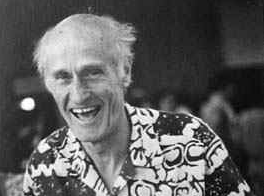
\includegraphics[width=\textwidth]{images/Kleene.png}    
\end{center}

\end{column}

\begin{column}{0.75\textwidth}

En septiembre de 1935 \textit{Kleene} presentó en una comunicación donde definió \textbf{las funciones recursivas primitivas} y las \textbf{funciones recursivas generales}  y demostraba el teorema de la Forma Normal donde demostró que cada programa admite uno equivalente usando bucles FOR y un sólo bucle WHILE.\\



\end{column}
\end{columns}


\begin{columns}
\begin{column}{0.15\textwidth}

\begin{center}
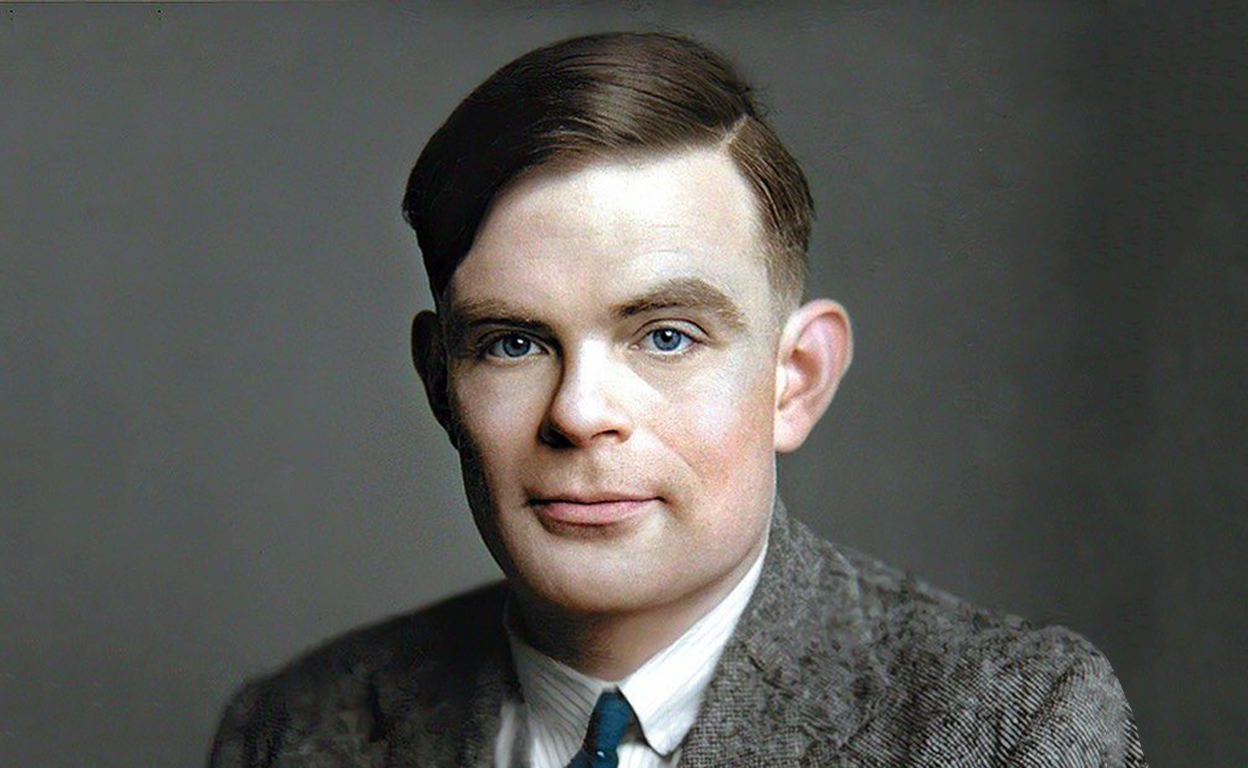
\includegraphics[width=\textwidth]{images/alan-turing-segunda-guerra-mundial-codigo-enigma-espia-f.jpg}    
\end{center}

\end{column}

\begin{column}{0.75\textwidth}


En 1936 \textit{Alan Turing} (1912-1954) da una nueva formalización definiendo lo que hoy se conoce como máquina de Turing. Turing entre otros elementos trató \textbf{el problema de la parada}, definió el concepto de ``\textbf{paso de cómputo}'', el cual es fundamental para el desarrollo de la teoría de la complejidad.

\end{column}
\end{columns}

\begin{columns}
\begin{column}{0.15\textwidth}

\begin{center}
\end{center}

\end{column}

\begin{column}{0.75\textwidth}

Posteriormente a los \textbf{modelos de Church, Kleene y Turing}, han aparecido otros con diferentes orientaciones.  Uno de ellos es el \textbf{lenguaje WHILE}, que tiene sentencias de asignación y una sola de control que le da nombre al lenguaje, el bucle WHILE.


\end{column}
\end{columns}
\hspace{3cm}



\end{frame}


%%%%%%%%%%%%%%%%%%%%%%%%%%%%%%%%
\begin{frame}[fragile]\frametitle{Formalización del concepto de algoritmo} \footnotesize

\begin{itemize}
    \item Según la \textbf{tesis de Church-Turing}, las \textbf{funciones computables} son exactamente las funciones que pueden calcularse utilizando un dispositivo de cálculo mecánico dadas cantidades ilimitadas de tiempo y espacio de almacenamiento. 
    \item  Equivalentemente, esta tesis afirma que una \textbf{función es computable} si y sólo si tiene un \textbf{algoritmo}.

    \begin{itemize}\footnotesize
        \item Así, podemos decir que un \textbf{algoritmo} es una secuencia finita de instrucciones precisas (no ambiguas) que, para un cierto tipo de entrada, o bien nos devuelve (computa en un tiempo finito) \textbf{una salida} o bien \textbf{no termina nunca}.
        
        \item Si un algoritmo siempre, para su tipo de entrada, nos devuelve en un tiempo finito una salida, entonces decimos que es un \textbf{algoritmo conclusivo}.
        
        \item Diremos que una \textbf{función} es \textbf{computable} si existe un algoritmo que para cualquier argumento de la función como entrada nos devuelve el valor de la función como salida. 
        
        \item Si la función para cierto argumento no toma valor (es decir, es una \textbf{función parcial}) entonces el \textbf{algoritmo} para ese argumento como entrada \textbf{no termina} nunca.
        
        \item De aquí se deduce que si una \textbf{función} computable es \textbf{total} entonces el algoritmo que la computa es un \textbf{algoritmo conclusivo}.
    \end{itemize}
\end{itemize}
\end{frame}

%%%%%%%%%%%%%%%%%%%%%%%%%%%%%%%%
\begin{frame}[fragile]\frametitle{Formalización del concepto de algoritmo} \small

\begin{itemize}
    \item Sea A un conjunto de cadenas sobre un alfabeto y B un subconjunto de A.

    \item Diremos que B es un \textbf{conjunto decidible} si existe un algoritmo conclusivo que dado un elemento de A como entrada nos dice siempre (en un tiempo finito al ser el algoritmo conclusivo) si dicho elemento pertenece o no al conjunto B .

    \item Diremos que B es un \textbf{conjunto enumerable} si existe un algoritmo que dado un elemento de A como entrada nos devuelve una respuesta afirmativa si y sólo si dicho elemento pertenece al conjunto B.

    \item La diferencia entre \textbf{decidible} y \textbf{enumerable} es que en el primer caso siempre tenemos respuesta del algoritmo, mientras que en el segundo sólo podemos asegurar que el algoritmo terminará si el elemento en cuestión pertenece al conjunto.

    \item De aquí se deduce que todo conjunto decidible es enumerable pero no a la inversa.
\end{itemize}

\end{frame}
%%%%%%%%%%%%%%%%%%%%%%%%%%%%%%%%%%%%%%%%%%%%%%%%%%%
%%%%%%%%%%%%%%%%%%%%%%%%%%%%%%%%%%%%%%%%%%%%%%%%%%%
%%%%%%%%%%%%%%%%%%%%%%%%%%%%%%%%%%%%%%%%%%%%%%%%%%%



%%%%%%%%%%%%%%%%%%%%%%%%%%%%%%%%%%%%%%%%%%%%%%%%%%%
%%%%%%%%%%%%%%%%%%%%%%%%%%%%%%%%%%%%%%%%%%%%%%%%%%%


\section{Lenguaje While}

\begin{chapter}[images/etsiinformatica4.png]{uicblue}{Lenguaje While}
\end{chapter}


%%%%%%%%%%%%%%%%%%%%%%%%%%%%%%%%%%%%%%%%%%%%%%%%%%%
%%%%%%%%%%%%%%%%%%%%%%%%%%%%%%%%%%%%%%%%%%%%%%%%%%%
%%%%%%%%%%%%%%%%%%%%%%%%%%%%%%%%
\subsection{Concepto informal}
\begin{frame}  \Large

\begin{center}
    \textbf{Concepto informal}
\end{center}

\end{frame} 
%%%%%%%%%%%%%%%%%%%%%%%%%%%%%%%%
\begin{frame}[fragile]\frametitle{Concepto informal} \small  
Para formalizar el concepto de función computable (WHILE-computable) definimos previamente un modelo de cómputo el lenguaje WHILE.

\begin{itemize}
    \item El lenguaje WHILE se puede entender como un lenguaje de programación muy simplificado.

    \item Sólo trabaja con naturales
    
\end{itemize}
\end{frame}

%%%%%%%%%%%%%%%%%%%%%%%%%%%%%%%%
\begin{frame}[fragile]\frametitle{Concepto informal} \small  

\begin{itemize}
    \item \textbf{Cuatro tipos de sentencias} de asignación,
        \begin{itemize}
        \item ${X_i}$ := 0 asignar a una variable la constante cero
        \item ${X_i}$ := ${X_j}$ asignar a una variable el valor de otra variable,
        \item ${X_i}$ := ${X_j}$ + 1 asignar a una variable el valor de otra variable incrementada en una unidad,
        \item ${X_i}$ := ${X_j}$ - 1 y asignar a una variable el valor de otra variable decrementada en una unidad.
        \end{itemize}

  \item Un \textbf{tipo de sentencia de control.} condición valor de una variable (denominada de control) es distinto de cero.
        \begin{itemize}
            \item while $X_i \neq 0$ x do (es la llamada cabecera del bucle)
            \item código (es el llamado cuerpo del bucle)
            \item od (es la llamada cola del bucle)
        \end{itemize}

\end{itemize}
\end{frame}

%%%%%%%%%%%%%%%%%%%%%%%%%%%%%%%%
\begin{frame}[fragile]\frametitle{Concepto informal} \small  

\begin{itemize}
    \item En un programa WHILE los identificadores de variables tienen la forma: $X_1$ , $X_2$ , $X_3$, $\ldots$, $X_i$, $\ldots$
  \item  Un código es una \textbf{secuencia finita no vacía de sentencias} separadas por el símbolo ``;''.
  \item  Un programa WHILE es una terna (n, p, s) donde

  \begin{itemize}
    \item  $n$ y $p$ son naturales con $p \geq n$ y $p > 0$;
    \item s es un código según la sintaxis anteriormente descrita.

\end{itemize}

\end{itemize}
\end{frame}


%%%%%%%%%%%%%%%%%%%%%%%%%%%%%%%%
\begin{frame}[fragile]\frametitle{Concepto informal} \small  

Un programa WHILE (n, p, s) esto significa que el programa tiene:


\begin{itemize}
    \item p \textbf{variables de uso en total} ($X_1$ , $X_2$ , $X_3$ , $\ldots$ , $X_p$ ) que toman valores naturales, de ellas:
    \item n son \textbf{variables de entrada} ($X_1$ , $X_2$ , $X_3$  , $\ldots$ , $X_n$ ), denominándose a
    \item p-n las restantes \textbf{variables auxiliares}. Se inicializan implícitamente a cero al inicio de la ejecución del programa.
    \item No hay instrucciones de entrada ni de salida.
    \item La salida del programa es el valor de la variable $X_1$ cuando el programa termina
\end{itemize}
\end{frame}


%%%%%%%%%%%%%%%%%%%%%%%%%%%%%%%%
\begin{frame}[fragile]\frametitle{Concepto informal} \small  

El funcionamiento de un programa WHILE consiste, dado que es un modelo basado en un lenguaje estructurado, en ejecutar secuencialmente las sentencias que componen su código, empezando por la primera del mismo.

\begin{itemize}
    \item Se ejecuta una sentencia cuando la anterior ha sido terminada.
    \item La sentencia de \textbf{decremento} ( $X_i := X_j - 1$ ) asigna el valor cero a la variable resultante en el caso de que la variable decrementada valiera cero antes de la sentencia.
    
    \item  Respecto a la sentencia de control (while), ésta primero comprueba si la variable de control que aparece en su cabecera es distinta de cero; si es así ejecutará el código que compone el cuerpo del bucle, tras lo cual volverá a comprobar la variable. Esto se repetirá mientras dicha variable sea distinta de cero cada vez que sea comprobada.

\end{itemize}

\end{frame}

%%%%%%%%%%%%%%%%%%%%%%%%%%%%%%%%
\begin{frame}[fragile]\frametitle{Concepto informal} \small  


\begin{itemize}
    \item  Respecto a la sentencia de control (while), ésta primero comprueba si la variable de control que aparece en su cabecera es distinta de cero; si es así ejecutará el código que compone el cuerpo del bucle, tras lo cual volverá a comprobar la variable. Esto se repetirá mientras dicha variable sea distinta de cero cada vez que sea comprobada.
    \item Si en una de las comprobaciones vale cero la sentencia while termina.
    \item Podemos por tanto asociar una única función de $N^n$ en N a cada programa WHILE, \textbf{función calculada por un programa WHILE}.
    \item Función puede ser \textbf{parcial}, ya que puede haber entradas para las cuales el programa no termina (diverge).
\end{itemize}

\end{frame}

%%%%%%%%%%%%%%%%%%%%%%%%%%%%%%%%
\begin{frame}[fragile]\frametitle{Ejemplo} \small  

\begin{block}{}

Sea Q = (1, 2, s) con s: \hfill \break
$X_2 := X_1$;\\
while $X_2 \neq 0$ do\\
\hspace{0.5cm}$X_1$ := $X_1 + 1$;\\
\hspace{0.5cm}$X_2$ := $X_2 - 1$\\
od
\end{block}

\end{frame}

%%%%%%%%%%%%%%%%%%%%%%%%%%%%%%%%%%%%%%%%%%%%%%%%%%%
%%%%%%%%%%%%%%%%%%%%%%%%%%%%%%%%%%%%%%%%%%%%%%%%%%%

%%%%%%%%%%%%%%%%%%%%%%%%%%%%%%%%%%%%%%%%%%%%%%%%%%%
%%%%%%%%%%%%%%%%%%%%%%%%%%%%%%%%%%%%%%%%%%%%%%%%%%%
%%%%%%%%%%%%%%%%%%%%%%%%%%%%%%%%
\subsection{Concepto formal}

\begin{frame}  \Large

\begin{center}
    \textbf{Concepto formal: Sintáxis}
\end{center}

\end{frame} 

%%%%%%%%%%%%%%%%%%%%%%%%%%%%%%%%
\begin{frame}[fragile]\frametitle{Concepto formal:Sintáxis} \small  

Tenemos dos alfabetos:
\begin{itemize}
    \item $\Sigma_d$ = \{ 0 , 1 , 2 , 3 , 4 , 5 , 6 , 7 , 8 , 9 \}. El alfabeto $\Sigma_d$ está formado por los dígitos en subíndice.

    \item $\Sigma_1$ = \{ X , := , + , - , 1 , while , $\neq$ , 0 , do , od , ; \} ``while'' es un solo símbolo perteneciente al alfabeto $\Sigma_1$, que tiene por tanto once símbolos.
\end{itemize}


\end{frame}

%%%%%%%%%%%%%%%%%%%%%%%%%%%%%%%%
\begin{frame}[fragile]\frametitle{Concepto formal: Sintáxis} \small  

Tenemos dos gramáticas:\hfill \break

Sea $G_1$ = ( $N_1$ , $T_1$ , $P_1$ , <número> ) una gramática con:\\
\vspace{0.1cm}
$N_1$ = \{ <número> , <p\_dígito> , <r\_número> , <dígito> \}\\
\vspace{0.1cm}
$T_1$ = $\Sigma_d$\\
\vspace{0.1cm}
$P_1$ = \{<número> $\rightarrow$ <p\_dígito>\break
\vspace{0.1cm}
\hspace{2.5cm} | <p\_dígito> <r\_número>,\break
\vspace{0.1cm}
\hspace{0.5cm}<p\_dígito> $\rightarrow$ 1 | 2 | 3 | 4 | 5 | 6 | 7 | 8 | 9,\break
\vspace{0.1cm}
\hspace{0.5cm}<r\_número> $\rightarrow$ <dígito>\break
\vspace{0.1cm}
\hspace{2.5cm} | <dígito> <r\_número>,\break
\vspace{0.1cm}
\hspace{0.5cm} <dígito> $\rightarrow$ 0 | 1 | 2 | 3 | 4 | 5 | 6 | 7 | 8 | 9 \}\break

\end{frame}

%%%%%%%%%%%%%%%%%%%%%%%%%%%%%%%%
\begin{frame}[fragile]\frametitle{Concepto formal: Sintáxis} \footnotesize  


Sea $G_2$ = ( $N_2$ , $T_2$ , $P_2$ , <código> ) una gramática con:\hfill \break
\vspace{0.1cm}
$N_2$ = \{ <código>, <sentencia>, <asignación>, <bucle>, <identificador> \} $\cup$ $N_1$ \break
\vspace{0.1cm}
$T_2$ = $\Sigma_d$ $\cup$ $\Sigma_1$\break
\vspace{0.1cm}
$P_2$ = \{ <código> $\rightarrow$ <sentencia>\break
\vspace{0.1cm}
\hspace{2.1cm} | <código> ; <sentencia>,\break
\vspace{0.1cm}
\hspace{0.8cm}<sentencia> $\rightarrow$ <asignación>\break
\vspace{0.1cm}
\hspace{2.5cm} | <bucle> ,\break
\vspace{0.1cm}
\hspace{0.8cm}<asignación> $\rightarrow$ <identificador> := 0\break
\vspace{0.1cm}
\hspace{2.8cm}| <identificador> := <identificador>\break
\vspace{0.1cm}
\hspace{2.8cm}| <identificador> := <identificador> + 1\break
\vspace{0.1cm}
\hspace{2.8cm}| <identificador> := <identificador> - 1,\break
\vspace{0.1cm}
\hspace{0.8cm}<bucle> $\rightarrow$ while <identificador> $\neq 0$ do <código> od,\break
\vspace{0.1cm}
\hspace{0.8cm}<identificador> $\rightarrow$ X<número> \} $\cup$ $P_1$

\end{frame}

%%%%%%%%%%%%%%%%%%%%%%%%%%%%%%%%
\begin{frame}[fragile]\frametitle{Concepto formal: Sintáxis} \small  

\begin{block}{Definición 1: Código While, Conjunto de códigos While (Cód\_While)}
\end{block}
Sea s $\in$ $T^+_2$. Diremos que s es un código While sii s $\in$ L($G_2$).\break
\vspace{0.2cm}
El conjunto de códigos While, notado Cód\_While, se define como: Cód\_While = L($G_2$).\hfill \break
\scriptsize
Nota: El conjunto Cód\_While está formado por todos los códigos en lenguaje WHILE sintácticamente correctos.\small


\begin{block}{Definición 2: Programa WHILE, Conjunto de programas WHILE (WHILE)}
\end{block}
El conjunto de programas WHILE, notado WHILE , se define como:
\begin{center}
WHILE = \{ (n, p, s) $\in$ N x N x Cód\_While | $p \geq n$ $\wedge$ p > 0 $\wedge$ ( $X_m$ $\succ$ s con m $\in$ $\Sigma^+_d$ $\Rightarrow$  $m \leq  p$ ) \} 
\end{center}

Diremos que Q es un programa WHILE sii Q $\in$ WHILE.
\hfill \break
\scriptsize
Nota: La expresión ``$X_m \succ$ s” significa que la cadena ``$X_m$'' es subcadena de la cadena ``s''. 

\end{frame}


%%%%%%%%%%%%%%%%%%%%%%%%%%%%%%%%%%%%%%%%%%%%%%%%%%%
%%%%%%%%%%%%%%%%%%%%%%%%%%%%%%%%%%%%%%%%%%%%%%%%%%%
%%%%%%%%%%%%%%%%%%%%%%%%%%%%%%%%
\subsection{Semántica}

\begin{frame}  \Large

\begin{center}
    \textbf{Concepto formal: Semántica}
\end{center}

\end{frame} 

%%%%%%%%%%%%%%%%%%%%%%%%%%%%%%%%
\begin{frame}[fragile]\frametitle{Concepto formal: Semántica} \small  

\begin{block}{Definición 3: Tamaño de un código While (tam)}
\end{block}
Sea s $\in$ Cód\_While, definimos el tamaño de s , notado \textit{tam(s)}, como:


\begin{itemize}
    \item Si en $G_2$ se cumple que <asignación> $\Rightarrow^*$ s, entonces: tam(s) = 1

    \item Si s = while $X_i \neq 0$ do $s_1$ od , con i$\in$ $\Sigma_d^+$
y $s_1$ $\in$ Cód\_While , entonces: tam(s) = tam($s_1$) + 2

    \item Si s = $s_1$ ; $s_2$ , con $s_1$, $s_2$ $\in$ Cód\_While, entonces: tam(s) = tam($s_1$) + tam($s_2$)
\end{itemize}



\begin{block}{Definición 4: Tamaño de un programa WHILE (tam)}
\end{block}

Sea Q $\in$ WHILE , con Q = (n, p, s) . Definimos el tamaño de Q, notado tam(Q) , como: tam(Q) = tam(s)

\end{frame}

%%%%%%%%%%%%%%%%%%%%%%%%%%%%%%%%
\begin{frame}[fragile]\frametitle{Volvemos con el Ejemplo} \small  
\footnotesize
\begin{block}{}Sea Q = (1, 2, s) con s: \hfill \break
$X_2 := X_1$;\\
while $X_2 \neq 0$ do\\
\hspace{0.5cm}$X_1$ := $X_1 + 1$;\\
\hspace{0.5cm}$X_2$ := $X_2 - 1$\\
od
\end{block}


\begin{center}
 WHILE = \{ (n, p, s) $\in$ N x N x Cód\_While | $p \geq n$ $\wedge$ p > 0 $\wedge$ ($X_m$ 
 $\succ$ s con m $\in$ $\Sigma^+_d$  $\Rightarrow$  m $\leq$  p) \}
 \end{center}

Q $\in$ WHILE , es decir, es un programa WHILE, ya que se cumple que:\\
\hspace{0.5cm}Q $\in$ N x N x Cód\_While $\wedge$ 2 $\geq$ 1 $\wedge$ p $\geq$ n $\wedge$ 2 > 0 $\wedge$  p > 0 $\wedge$ ($X_m$ $\succ$  s con m $\in$ $\Sigma_d^+$ $\Rightarrow$ m $\leq$ 2 ) \\
\hfill \break
\footnotesize
El hecho de que la tercera componente de Q, es decir, la cadena s, pertenezca a Cód\_While
\begin{itemize}
    \item significa que s es un código en lenguaje WHILE sintácticamente correcto,
    \item cumpliéndose que tam(Q)=tam(s)=5
\end{itemize}


\end{frame}

%%%%%%%%%%%%%%%%%%%%%%%%%%%%%%%%
\begin{frame}[fragile]\frametitle{Función Línea ...} \footnotesize
\begin{block}{Definición 5: Función línea...} 
\end{block}

Definimos la función \textbf{línea} : Cód\_While x $N$ $\rightarrow$ $T_2^*$ como:

\begin{enumerate}
    \item Si en $G_2$ se cumple que <asignación> $\Rightarrow^*$ s, entonces:
    
    \scriptsize\begin{equation*} linea(s,n) = \begin{cases} s & \text{si n=1}\\\epsilon &\text{en\:otro\:caso} \end{cases} \end{equation*}

    \item Si s = while $X_i$ $\neq$ 0 do $s_1$ od, con $i \in \Sigma_d^+$ y $s_1 \in$ Cód\_While, entonces:

    \scriptsize\begin{equation*} linea(s,n) = 
    \begin{cases} 
            while\; X_i \neq 0 \;do & \text{si n=1}\\
            od                      & \text{si\; n =tam(s)}\\
             linea(s_1,n-1)         &  si\; 1 <n<tam(s) \\ 
            \epsilon                & \text{en\:otro\:caso}
    \end{cases} \end{equation*}

   
        
\end{enumerate}


\end{frame}

%%%%%%%%%%%%%%%%%%%%%%%%%%%%%%%%
\begin{frame}[fragile]\frametitle{... Función Línea} \footnotesize
\begin{block}{Definición 5: .. Función línea}
\end{block}

\begin{enumerate}
    \setcounter{enumi}{2}
    \item Si s = s1 ; s2 , con s1 , s2 $\in$ Cód\_While , entonces:

         \scriptsize\begin{equation*} linea(s,n) = 
            \begin{cases} 
                    linea(s_1,n)            & \text{si 0 < n $\leq$ tam ($s_1$)}\\
                    linea(s_2,n-tam(s_1))   & \text{si\; tam($s_1$) <n $\leq$ tam (s) }\\
                    \epsilon                & \text{en\:otro\:caso}
            \end{cases} \end{equation*}   
        
\end{enumerate}


Nota: La función línea devuelve el texto de una línea concreta de un código While, o bien la cadena vacía si el número de
línea no es válido.

\end{frame}

%%%%%%%%%%%%%%%%%%%%%%%%%%%%%%%%
\begin{frame}[fragile]\frametitle{Función salto...} \footnotesize
\begin{block}{Definición 6: Función salto...} 
\end{block}

Definimos la función \textbf{salto} : Cód\_While x N $\rightarrow$ N como:

\begin{enumerate}
     \item Si en $G_2$ se cumple que <asignación> $\Rightarrow^*$ s, entonces: salto(s,n) = 0

      \item Si s = while $X_i$ $\neq$ 0 do $s_1$ od, con $i \in \Sigma_d^+$ y $s_1 \in$ Cód\_While, entonces:

         \scriptsize\begin{equation*} salto(s,n) = 
            \begin{cases} 
                    tam(s)+1              & \text{si n=1}\\
                    1                     & \text{si\; n =tam(s)}\\
                    salto(s_1,n-1)+1      & si\; (1<n<tam(s)) \wedge (salto(s_1,n-1) \neq 0) \\
                    0                     & \text{en\:otro\:caso}
            \end{cases} \end{equation*}   
        
\end{enumerate}

\end{frame}
%%%%%%%%%%%%%%%%%%%%%%%%%%%%%%%%
\begin{frame}[fragile]\frametitle{...  Función salto} \footnotesize
\begin{block}{Definición 6: .. Función salto}
\end{block}

\begin{enumerate}
    \setcounter{enumi}{2}
    \item Si s = s1 ; s2 , con s1 , s2 $\in$ Cód\_While , entonces:

         \scriptsize\begin{equation*} salto(s,n) = 
            \begin{cases} 
                    salto(s_1,n)            & 0< n \leq tam(s_1)\\
                    salto(s_2,n-tam(s_1))+tam(s_1))   & si\; (tam(s_1) < n \leq tam (s)) \wedge (salto (s_2,n-tam(s_1))\neq 0) \\
                    0                & \text{en\:otro\:caso}
            \end{cases} \end{equation*}   
        
\end{enumerate}


Nota: La función salto devuelve \textcolor{red}{el número de línea no consecutiva} al que se podría saltar desde una \textbf{línea dada} (N) de un \textbf{código While} (Cód\_While), o bien \textcolor{red}{cero} si desde la línea especificada no se puede saltar a una línea no consecutiva.

\end{frame}

%%%%%%%%%%%%%%%%%%%%%%%%%%%%%%%%%%%%%%%%%%%%%%%%%%%
%%%%%%%%%%%%%%%%%%%%%%%%%%%%%%%%%%%%%%%%%%%%%%%%%%%
%%%%%%%%%%%%%%%%%%%%%%%%%%%%%%%%
\begin{frame}  \Large

\begin{center}
    \textbf{Preguntas\\ Definición, tamaño, línea y salto }
\end{center}

\end{frame} 


%%%%%%%%%%%%%%%%%%%%%%%%%%%%%%%%
\begin{frame}[fragile]\frametitle{Preguntas} \footnotesize

\begin{enumerate}\footnotesize
    \item ¿$ (1,2,X_3:=0) \in WHILE?$\\
    \hspace{0.3cm} \scriptsize  \textcolor{chicagoblue}{No.	Un	programa	con	dos	variables	en	total	no	puede	tener	la	variable	$X_3$ en	su	código.}
    \footnotesize
    \item ¿Un	programa	WHILE	puede	tener	infinitas	variables?\\
        \hspace{0.3cm} \scriptsize \textcolor{chicagoblue}{No.	Por	definición,	la	segunda	componente	de	la	terna	que	define	un	programa	WHILE,	que	indica	cuantas	variables tiene	el	programa,	es	un	natural,	por	lo	que	el	número	de	variables	siempre	es	finito.}
    \footnotesize
    
    \item ¿Si	s	=	$s_1$	;	$s_2$	con	$s_1$,	$s_2$	$\in$ Cód\_WHILE	entonces	tam(s)	>	tam($s_1$)	?\\
        \hspace{0.3cm} \scriptsize \textcolor{chicagoblue}{Sí.	Puesto	que	un	código	siempre	tiene	al	menos	tamaño	uno (según	definición	por	la	gramática),	y	el	tamaño	de	una	 secuencia	es	la	suma	de	los	tamaños	de	sus	códigos.}
    \footnotesize
    \item ¿	tam(s)	>	n	$\rightarrow$ línea(s,	n)	=	0	?\\
        \hspace{0.3cm} \scriptsize \textcolor{chicagoblue}{No.	 La	 función	 línea	 nunca	 devuelve	 cero.	 Devuelve	 el	 texto	 de	 una	 línea	 concreta	 de	 un	 código	 While,	 o	 bien	 la	 cadena	vacía	si	el	número	de	línea	no	es	válido.}
    \footnotesize
    \item ¿	n $\in$ N-\{0\} $\wedge$ $\exists$ s $\in$ Cód\_While |	salto(s,n)	=	n	? \\
       \hspace{0.3cm}  \scriptsize \textcolor{chicagoblue}{No.	La	función	salto,	por	definición,	nunca	devuelve	la	misma	línea	de	la	que	parte.}
       
\end{enumerate}


\end{frame}

%%%%%%%%%%%%%%%%%%%%%%%%%%%%%%%%%%%%%%%%%%%%%%%%%%%
%%%%%%%%%%%%%%%%%%%%%%%%%%%%%%%%%%%%%%%%%%%%%%%%%%%
%%%%%%%%%%%%%%%%%%%%%%%%%%%%%%%%


%%%%%%%%%%%%%%%%%%%%%%%%%%%%%%%%
\begin{frame}[fragile]\frametitle{Configuración,Conjunto de configuraciones } \small  

\begin{block}{Definición 7: Configuración,Conjunto de configuraciones}
\end{block}
Sea Q $\in$ WHILE, con Q=(n,p,s). Definimos el \textcolor{red}{conjunto de configuraciones} de Q, notado como $C_Q$ como:

\begin{center}
$C_Q$ = \{ \underline{c} $\in$ $N^{p+1}$ | \underline{c} = (m, \underline{x}) con 1 $\leq$ m $\leq$ tam(Q)+1 y \underline{x} $\in$ $N^p$\}
\end{center}

Diremos que \underline{c} es una \textcolor{red}{configuración} de Q sii c $\in$ $C_Q$.

\vspace{1cm}

\footnotesize Nota: La configuración nos indica la posición en el código while y el estado de las variables del programa.
\end{frame}

%%%%%%%%%%%%%%%%%%%%%%%%%%%%%%%%
\begin{frame}[fragile]\frametitle{ Configuración inicial, terminal} \footnotesize  

\begin{block}{Definición 8: Configuración inicial}
\end{block}


Sea Q $\in$ WHILE, con Q=(n,p,s),  y sea \underline{c} $\in C_Q$, con \underline{c} = (m, \underline{x}). Diremos que \underline{c} es \textcolor{red}{configuración inicial}  de Q sii

\begin{center}
m = 1 $\wedge$ $x_{n+1}$ = $\ldots$ = $x_p$ = 0
\end{center}
\vspace{0.1cm}

\scriptsize Nota: Los valores de las variables que no son de entrada, son ceros.


\begin{block}{Definición 9: Configuración terminal, Configuración no terminal }
\end{block}

Sea Q $\in$ WHILE,  y sea \underline{c} $\in C_Q$, con \underline{c} = (m, \underline{x}). \\

- Diremos que \underline{c} es \textcolor{red}{configuración terminal} de Q sii m= tam(Q) +1.\\
- En caso contrario decimos que es una \textcolor{red}{configuración no terminal}.

\end{frame}

%%%%%%%%%%%%%%%%%%%%%%%%%%%%%%%%
\begin{frame}[fragile]\frametitle{Transitar directamente} \footnotesize  

\begin{block}{Definición 10: Transitar directamente}
\end{block}

Sea Q $\in$ WHILE, con Q=(n,p,s). Sean \underline{$c_1$}, \underline{$c_2$} $\in C_Q$, con \underline{$c_1$} = (m, \underline{x}) y  \underline{$c_2$} = (t, \underline{z}). Diremos que Q  \textcolor{red}{transita directamente} de   \underline{$c_1$}  a  \underline{$c_2$}, notado como  \underline{$c_1$} 
$\vdash$ \underline{$c_2$}, sii:\\
%\vspace{0.2cm}

\begin{columns}
\begin{column}{0.43\textwidth}
\hspace{2cm}    \textbf{Asignaciones}
\begin{colorblock}[white]{uihteal}{}
linea(s,m) = $X_i$ :=0 con i $\in$ $\Sigma_d^+$\\
\hspace{0.5cm} $\Rightarrow$ t = m+1 $\wedge$ $z_i$=0 $\wedge$ ($z_r$ = $x_r$ $\forall$ r $\neq$ i) 

linea(s,m) = $X_i$ := $X_j$  con i $\in$ $\Sigma_d^+$\\
\hspace{0.5cm} $\Rightarrow$ t = m+1 $\wedge$ $z_i$= $z_j$ $\wedge$ ($z_r$ = $x_r$ $\forall$ r $\neq$ i) 

linea(s,m) = $X_i$ := $X_j+1$ con i $\in$ $\Sigma_d^+$\\
\hspace{0.5cm} $\Rightarrow$ t = m+1 $\wedge$ $z_i$= $z_j+1$ $\wedge$ ($z_r$ = $x_r$ $\forall$ r $\neq$ i) 

linea(s,m) = $X_i$ := $X_j-1$ con i $\in$ $\Sigma_d^+$\\
\hspace{0.5cm} $\Rightarrow$ t = m+1 $\wedge$ $z_i$= $z_j-1$ $\wedge$ ($z_r$ = $x_r$ $\forall$ r $\neq$ i) 
\end{colorblock}
\end{column}



\begin{column}{0.6\textwidth}

\begin{center}
    \textbf{While/od}
\end{center}

\begin{colorblock}[white]{uihteal}{}
linea(s,m) = while $X_i$ $\neq$ 0 do con i $\in$ $\Sigma_d^+$\\
\hspace{0.3cm} $\Rightarrow$ ($x_i$ $\neq$ 0 $\Rightarrow$ t = m+1) 
$\wedge$ ($x_i$=0 $\Rightarrow$ t = salto(s,m)) $\wedge$ ( \underline{$z$} =  \underline{$x$} ) 

linea(s,m) = od \\
\hspace{0.3cm} $\Rightarrow$ t = salto (s,m) $\wedge$ ( \underline{$z$} =  \underline{$x$} ) 
\end{colorblock}

\end{column}
\end{columns}
\end{frame}

%%%%%%%%%%%%%%%%%%%%%%%%%%%%%%%%
\begin{frame}[fragile]\frametitle{Ejemplo 1} \footnotesize  

\begin{columns}

    \begin{column}{0.4\textwidth}
        \begin{colorblock}[black]{championsgold}{}\scriptsize
        Sea Q = (1, 2, s) con s: \\
        \hspace{0.5cm}   $X_2$ := $X_1$;\\
        \hspace{0.5cm}   while $X_2$ $\neq$ 0 do \\
        \hspace{0.75cm}    $X_1$ := $X_1$ + 1;\\
        \hspace{0.75cm}    $X_2$ := $X_2$ - 1\\
        \hspace{0.5cm}  od
        \end{colorblock}
        \end{column}

    \begin{column}{0.43\textwidth}
        \begin{colorblock}[white]{steelgray}{}\scriptsize
           \begin{center}
               \textit{¡¡ Recuerda !!} \\
           \end{center} 
            \textbf{Configuraciones} \underline{c} = (m,\underline{x})\\
            \textbf{Inicial}: m=1 $\wedge$ $x_{n+1}$ = $\ldots$  $x_p$ = 0\\
            \textbf{Terminal}: sii m = tam (Q) +1
            \end{colorblock}
    \end{column}

    
    
\end{columns}


\begin{itemize}
\scriptsize
    \item El vector (1,1,1) es una configuración de Q , es decir, (1,1,1) $\in$ $C_Q$.

        \begin{itemize}   \tiny
            \item \textcolor{red}{No es una configuración inicial}, ya que la tercera componente no es cero.
            \item \textcolor{red}{No es terminal}, , puesto que la primera componente no es seis. (tam(Q) +1 = 6)
            \item (1,1,1) $\vdash$ (2,1,1), es decir, Q transita directamente de (1,1,1) a (2,1,1)
        \end{itemize}

 \item El vector (0,1,1) \textcolor{red}{no es una configuración}  de Q ,
        \begin{itemize}   \tiny
            \item (0,1,1) $\notin$ $C_Q$ , ya que 0 $\notin$ [1, 6] .
            \item  no transita directamente a ninguna configuración, ya que no es una configuración
        \end{itemize}

    \item El vector (1,10,0) $\in$ $C_Q$, \\
      \hspace{0.3cm}      \tiny Siendo además \textcolor{red}{configuración inicial}. (1,10,0) $\vdash$  (2,10,10)
            
       \scriptsize     
    \item El vector (6,6,6) $\in$ $C_Q$,\\
      \hspace{0.3cm}       \tiny Siendo además  \textcolor{red}{configuración terminal}. Al ser terminal, no transita directamente a ninguna otra.
        
\end{itemize}

\end{frame}

%%%%%%%%%%%%%%%%%%%%%%%%%%%%%%%%%%%%%%%%%%%%%%%%%%%
%%%%%%%%%%%%%%%%%%%%%%%%%%%%%%%%%%%%%%%%%%%%%%%%%%%
%%%%%%%%%%%%%%%%%%%%%%%%%%%%%%%%
\begin{frame}  \Large

\begin{center}
    \textbf{Preguntas\\
    Configuraciones y Trancisiones}
\end{center}

\end{frame} 


%%%%%%%%%%%%%%%%%%%%%%%%%%%%%%%%
\begin{frame}[fragile]\frametitle{Preguntas} \footnotesize

\begin{enumerate}\footnotesize
    \item ¿Algún	programa	WHILE	tiene	un	número	finito	de	configuraciones	iniciales?\\
    \hspace{0.3cm} \scriptsize  \textcolor{chicagoblue}{Para que las configuraciones sean infinitas dependen del número de línea y del valor de las variables de entrada. Cómo el número de líneas es finito, solo depende de las variables de entrada. Si tiene una variable de entrada ya sería infinita. Solo sería finita si no tuviera variables de entrada.}
    \footnotesize
    \item Una	configuración	de	un	programa	WHILE	puede	ser	a	la	vez	inicial	y	terminal?\\
        \hspace{0.3cm} \scriptsize \textcolor{chicagoblue}{No. Ya que la configuraciones tienen como primera componente el número de línea en el que está el programa. Las configuraciones iniciales tienen un valor de 1, mientras que las finales tienen uno mas del tamaño del programa. Como el programa no puede ser vacío tendrá que tener al menos valor 2. }
    \footnotesize
    
    \item ¿$c_1$ $\vdash$ $c_2$ $\Rightarrow$  $c_1 \neq c_2$ ?\\
        \hspace{0.3cm} \scriptsize \textcolor{chicagoblue}{Sí.	El número de línea cambia de una configuración a su siguiente, mayor o menor, pero nunca igual.}
    
       
\end{enumerate}


\end{frame}


%%%%%%%%%%%%%%%%%%%%%%%%%%%%%%%%
\begin{frame}[fragile]\frametitle{ Función siguiente (SIG)  } \footnotesize  

\begin{block}{Definición 11: Función siguiente (SIG)}
\end{block}

Sea Q $\in$ WHILE, con Q=(n,p,s). Sea $C_Q$ el conjunto de configuraciones de Q. Definimos la función siguiente de Q, notada $SIG_Q$, como: $SIG_Q: N^{p+1} \rightarrow N^{p+1}$


   \scriptsize\begin{equation*} SIG_Q(\underline{c}) = 
            \begin{cases} 
                    \underline{c}'      & si\; \underline{c} \vdash  \underline{c}' \;con \;\underline{c}, \underline{c}' \in C_Q\\
                     \underline{c}      & si\; \nexists \; \underline{c}' \in C_Q |\; \underline{c} \vdash  \underline{c}' \;con \;\underline{c} \in C_Q \\
                     \underline{c}      & si\; \underline{c} \notin C_Q 
            \end{cases} \end{equation*}   

\scriptsize Nota: Amplía el concepto ``transitar directamente'' dándonos una función total. Simplemente me quedo en la misma configuración si no hay una configuración siguiente o no es válida.

\end{frame}

%%%%%%%%%%%%%%%%%%%%%%%%%%%%%%%%
\begin{frame}[fragile]\frametitle{ Función cálculo (CAL) } \footnotesize  


\begin{block}{Definición 12: Función cálculo (CAL) }
\end{block}

Sea Q $\in$ WHILE, con Q=(n,p,s). Definimos la función cálculo de Q, notada $CAL_Q$, como $N^{n+1} \rightarrow N^{p+1}$.

 \scriptsize\begin{equation*} CAL_Q(\underline{x},i) = 
            \begin{cases} 
                    (1,\underline{x},\underline{0})      & si\; i=0 \\
                    SIG_Q (CAL_Q(\underline{x},i-1))      & si\; i>0 
            \end{cases} \end{equation*}   
            
\scriptsize Nota: $i \in N$, $\underline{x} \in N^n$ y $\underline{0} \in N^{p-n}$ 

\end{frame}

%%%%%%%%%%%%%%%%%%%%%%%%%%%%%%%%
\begin{frame}[fragile]\frametitle{Ejemplo 1} \footnotesize  


        \begin{colorblock}[black]{championsgold}{}\scriptsize
        Sea Q = (1, 2, s) con s: \\
        \hspace{0.5cm}   $X_2$ := $X_1$;\\
        \hspace{0.5cm}   while $X_2$ $\neq$ 0 do \\
        \hspace{0.75cm}    $X_1$ := $X_1$ + 1;\\
        \hspace{0.75cm}    $X_2$ := $X_2$ - 1\\
        \hspace{0.5cm}  od
        \end{colorblock}


\begin{columns}

    \begin{column}{0.4\textwidth}
        \begin{colorblock}[black]{championsgold}{}\scriptsize
        $SIG_Q$(1,1,1)=(2,1,1) \\
        $SIG_Q$(0,1,1)=(0,1,1) \\
        $SIG_Q$(7,1,1)=(7,1,1)\\
        $SIG_Q$(1,10,0)=(2,10,10)\\
        $SIG_Q$(6,6,6)=(6,6,6)\\
        \end{colorblock}
        \end{column}

    \begin{column}{0.43\textwidth}
        \begin{colorblock}[white]{steelgray}{}\scriptsize
           \scriptsize\begin{equation*} SIG_Q(\underline{c}) = 
            \begin{cases} 
                    \underline{c}'      & si\; \underline{c} \vdash  \underline{c}' \;con \;\underline{c}, \underline{c}' \in C_Q\\
                     \underline{c}      & si\; \nexists \; \underline{c}' \in C_Q |\; \underline{c} \vdash  \underline{c}' \;con \;\underline{c} \in C_Q \\
                     \underline{c}      & si\; \underline{c} \notin C_Q 
            \end{cases} \end{equation*}   
            \end{colorblock}
    \end{column}


\end{columns}

\end{frame}

%%%%%%%%%%%%%%%%%%%%%%%%%%%%%%%%
\begin{frame}[fragile]\frametitle{Ejemplo 1} \footnotesize  


        \begin{colorblock}[black]{championsgold}{}\scriptsize
        Sea Q = (1, 2, s) con s: \\
        \hspace{0.5cm}   $X_2$ := $X_1$;\\
        \hspace{0.5cm}   while $X_2$ $\neq$ 0 do \\
        \hspace{0.75cm}    $X_1$ := $X_1$ + 1;\\
        \hspace{0.75cm}    $X_2$ := $X_2$ - 1\\
        \hspace{0.5cm}  od
        \end{colorblock}


\begin{columns}

    \begin{column}{0.6\textwidth}
        \begin{colorblock}[black]{championsgold}{}\scriptsize
        $CAL_Q$(2,4) = \\
        $SIG_Q$( $CAL_Q$(2,3) ) = \\
        $SIG_Q$( $SIG_Q$( $CAL_Q$(2,2) ) ) = \\
        $SIG_Q$( $SIG_Q$( $SIG_Q$( $CAL_Q$(2,1) ) ) ) = \\
        $SIG_Q$( $SIG_Q$( $SIG_Q$($SIG_Q$($CAL_Q$(2,0) ) ) ) ) = \\
        $SIG_Q$( $SIG_Q$( $SIG_Q$( $SIG_Q$(1,2,0) ) ) ) = \textcolor{gray}{(1,2,0) |— (2,2,2)} \\
        $SIG_Q$( $SIG_Q$( $SIG_Q$(2,2,2) ) ) = \textcolor{gray}{(2,2,2) |— (3,2,2)} \\ %
        $SIG_Q$( $SIG_Q$(3,2,2) ) =  \textcolor{gray}{(3,2,2) |— (4,3,2)} \\ 
        $SIG_Q$(4,3,2) =  (5,3,1) \textcolor{gray}{(4,3,2) |— (5,3,1)} \\ 
        \end{colorblock}
        \end{column}

    \begin{column}{0.43\textwidth}
        \begin{colorblock}[white]{steelgray}{}\scriptsize
           \scriptsize\begin{equation*} CAL_Q(\underline{x},i) = 
            \begin{cases} 
                    (1,\underline{x},\underline{0})      & si\; i=0 \\
                    SIG_Q (CAL_Q(\underline{x},i-1))      & si\; i>0 
            \end{cases} \end{equation*}   
            \end{colorblock}
    \end{column}


\end{columns}

\end{frame}

%%%%%%%%%%%%%%%%%%%%%%%%%%%%%%%%
\begin{frame}[fragile]\frametitle{ Función complejidad temporal (T) } \footnotesize  


\begin{block}{Definición 13: Función complejidad temporal (T) }
\end{block}

Sea Q $\in$ WHILE, con Q=(n,p,s). 

Definimos la función complejidad de Q, notada $T_Q$, como $T_Q: N^{n} \rightarrow N$.

 \scriptsize\begin{equation*} T_Q(\underline{x}) = 
            \begin{cases} 
                    minimo(A)      & si\; A \neq  \varnothing\\
                    \uparrow       & si\; A =  \varnothing 
            \end{cases} \end{equation*}   

donde A= \{j $\in$ N | $\pi^{p+1}_1$ ( $CAL_Q$(\underline{x},j)) = tam (Q) +1) \}\\\break


\scriptsize $Nota_1$: $\pi^{3}_1$ (11, 22, 33) = 11. En nuestro caso el valor de la línea.\\
$Nota_2$: El Conjunto A está formado por todos los valores j que finalizan el programa.\\
$Nota_3$: Establece el número de la iteración que termina si existe, en caso contrario no termina.

\end{frame}

%%%%%%%%%%%%%%%%%%%%%%%%%%%%%%%%
\begin{frame}[fragile]\frametitle{Ejemplo 1} \footnotesize  

\begin{columns}

    \begin{column}{0.35\textwidth}
        \begin{colorblock}[black]{championsgold}{}\scriptsize
        Sea Q = (1, 2, s) con s: \\
        \hspace{0.5cm}   $X_2$ := $X_1$;\\
        \hspace{0.5cm}   while $X_2$ $\neq$ 0 do \\
        \hspace{0.75cm}    $X_1$ := $X_1$ + 1;\\
        \hspace{0.75cm}    $X_2$ := $X_2$ - 1\\
        \hspace{0.5cm}  od
        \end{colorblock}
 \end{column}

  \begin{column}{0.7\textwidth}
        \begin{colorblock}[white]{steelgray}{}\scriptsize
           $CAL_Q$(2,j) = 6 \\
           $SIG_Q$( $CAL_Q$(2,10) ) =\\
           $SIG_Q$( $SIG_Q$( $SIG_Q$( $SIG_Q$( $SIG_Q$( $SIG_Q$( $SIG_Q$( $SIG_Q$( $SIG_Q$( $SIG_Q$( $CAL_Q$(2,0) … ) =\\
          $\ldots$\\
           $SIG_Q$( (2,4,0 ))=\\
          (6,4,0 )

            \end{colorblock}
    \end{column}
\end{columns}
\begin{columns}

    \begin{column}{0.5\textwidth}
        \begin{colorblock}[black]{championsgold}{}\tiny
            \begin{table}[]
            \begin{tabular}{|l|l|l|l|}
            \hline\tiny
            \textbf{SIG} & \textbf{Línea} & \textbf{$X_1$} & \textbf{$X_2$} \\ \hline
            -                  & 1              & 2           & 0           \\ \hline
            1                  & 2              & 2           & 2           \\ \hline
            2                  & 3              & 2           & 2           \\ \hline
            3                  & 4              & 3           & 2           \\ \hline
            4                  & 5              & 3           & 1           \\ \hline
            5                  & 2              & 3           & 1           \\ \hline
            6                  & 3              & 3           & 1           \\ \hline
            7                  & 4              & 4           & 1           \\ \hline
            8                  & 5              & 4           & 0           \\ \hline
            9                  & 2              & 4           & 0           \\ \hline
            10                 & 6              & 4           & 0           \\ \hline
            \end{tabular}
            \end{table}
        \end{colorblock}
        \end{column}

    \begin{column}{0.43\textwidth}
        \begin{colorblock}[white]{steelgray}{}\scriptsize
           Función complejidad temporal al vector (2) tenemos: $T_Q$(2) = 10
            puesto que:\\
            mínimo \{ $j \in N$ | $\pi_1^3$ ($CAL_Q$(2, j)) = 6 \} = 10
            \end{colorblock}
    \end{column}


\end{columns}

\end{frame}


%%%%%%%%%%%%%%%%%%%%%%%%%%%%%%%%
\begin{frame}[fragile]\frametitle{ Función calculada (F) } \footnotesize  


\begin{block}{Definición 14: Función calculada (F)  }
\end{block}

Sea Q $\in$ WHILE, con Q=(n,p,s). 

Definimos la función calculada de Q, notada $F_Q$, como $F_Q: N^{n} \rightarrow N$.

\begin{center}
    $F_Q$ (\underline{x}) = $\pi_2^{p+1}$ ($CAL_Q$ ( \underline{x}, $T_Q$(\underline{x})))
\end{center}


\vspace{0.25cm}            
\scriptsize $Nota_1$: $\pi^{3}_2$ (11, 22, 33) = 22. En nuestro caso el valor de $X_1$.\\
\vspace{0.15cm}  
$Nota_2$: Aplicamos la función $CAL_Q$ el mínimo número de veces que necesitamos para el programa termine.\\
\vspace{0.15cm}  

\textbf{Ejemplo}:  (1,2,0) $\vdash$ (2,2,2) $\vdash$ (3,2,2) $\vdash$ (4,3,2) $\vdash$ (5,3,1) $\vdash$ (2,3,1) $\vdash$ (3,3,1) $\vdash$ (4,4,1) $\vdash$ (5,4,0) $\vdash$ (2,4,0) $\vdash$ (6,4,0). \\ 11 configuraciones, 10 transiciones

\end{frame}


%%%%%%%%%%%%%%%%%%%%%%%%%%%%%%%%%%%%%%%%%%%%%%%%%%%
%%%%%%%%%%%%%%%%%%%%%%%%%%%%%%%%%%%%%%%%%%%%%%%%%%%
%%%%%%%%%%%%%%%%%%%%%%%%%%%%%%%%
\begin{frame}  \Large

\begin{center}
    \textbf{Preguntas \\
    Función Calculada y complejidad Temporal}
\end{center}

\end{frame} 


%%%%%%%%%%%%%%%%%%%%%%%%%%%%%%%%
\begin{frame}[fragile]\frametitle{Preguntas} \footnotesize

\begin{enumerate}\footnotesize


    
    \item ¿$\forall Q \in WHILE\; \forall i \in N, CAL_Q(x,i) = CAL_Q (x,i+1) \Rightarrow T_Q(x) \leq i?$ \\
    \hspace{0.3cm} \scriptsize  \textcolor{chicagoblue}{Sí.	Si	dos	configuraciones	consecutivas	son	iguales	significa	que	en	ese	número	de	pasos,	o	menos,	el	programa	ya	ha terminado,	por	lo	que	acota	la	función	complejidad	temporal.}
    \footnotesize
    
    
    \item  ¿$\exists Q = (n,p,s) \in WHILE\; |\; T_Q(x) =0 \;con\; x \in N_N$?\\
        \hspace{0.3cm} \scriptsize \textcolor{chicagoblue}{No.	La	función	complejidad	temporal	o	bien	diverge,	o	bien	devuelve	un	natural	mayor	que	cero,	pero	nunca	puede devolver	cero	ya	que	todo	programa	ha	de	tener	alguna	sentencia.}
    \footnotesize
    
    \item ¿Si	Q	es	un	programa	WHILE	entonces	$F_Q$	diverge	si	y	sólo	si	$T_Q$	diverge?\\
        \hspace{0.3cm} \scriptsize \textcolor{chicagoblue}{Sí.	Dado	que	la	función	complejidad	temporal	nos	indica	en	cuantos	pasos	acaba	el	programa,	si	ella	es	total	la	
función	calculada	también,	y	si	ella	diverge	para	algún	valor,	para	ese	valor	la	función	calculada	también	diverge.}
    
       
\end{enumerate}


\end{frame}


%%%%%%%%%%%%%%%%%%%%%%%%%%%%%%%%%%%%%%%%%%%%%%%%%%%
%%%%%%%%%%%%%%%%%%%%%%%%%%%%%%%%%%%%%%%%%%%%%%%%%%%
%%%%%%%%%%%%%%%%%%%%%%%%%%%%%%%%
\begin{frame}  \Large

\begin{center}
    \textbf{Ejemplo 1 }
\end{center}

\end{frame} 



%%%%%%%%%%%%%%%%%%%%%%%%%%%%%%%%
\begin{frame}[fragile]\frametitle{Ejemplo 1} \footnotesize  


        \begin{colorblock}[black]{championsgold}{}\scriptsize
        Sea Q = (1, 2, s) con s: \\
        \hspace{0.5cm}   $X_2$ := $X_1$;\\
        \hspace{0.5cm}   while $X_2$ $\neq$ 0 do \\
        \hspace{0.75cm}    $X_1$ := $X_1$ + 1;\\
        \hspace{0.75cm}    $X_2$ := $X_2$ - 1\\
        \hspace{0.5cm}  od
        \end{colorblock}

    \begin{colorblock}[white]{steelgray}{}\tiny
       \scriptsize\begin{equation*} SIG_Q(\underline{c}) = 
        \begin{cases} 
                (0,b,c)    & si\; a =0  \;No\;es\; una\; configuraci\acute{o}n \;\underline{c} \notin C_0\\
                (2,b,b)    & si\; a =1  \;Asignaci\acute{o}n\; X_2 := X_1;\\
                (3,b,c)    & si\; a = 2 \wedge c \neq 0  \;Entra\; bucle\; c=0;\\
                (6,b,c)    & si\; a = 2 \wedge c = 0 Siguiente fuera bucle c=0\\
                (4,b+1,c)  & si\; a = 3 \;X1 := X1 + 1\\
                (5,b,c-1)  & si\; a = 4 \;X2 := X2 - 1\\
                (2,b,c)    & si\; a = 5 \;od\\
                (a,b,c)    & si\; a > 5 \;si  \;\nexists\; \underline{c}' \in C_Q\; |\;  c\; \vdash  \underline{c}'\; con \;\underline{c} \in C_Q
        \end{cases} \end{equation*}   
        \end{colorblock}

\end{frame}


%%%%%%%%%%%%%%%%%%%%%%%%%%%%%%%%
\begin{frame}[fragile]\frametitle{Ejemplo} \footnotesize  

Si comenzamos el cómputo con la configuración inicial (1, n, 0) , con n > 0 , tenemos:

\hspace{0.2cm} (1, n, 0) $\vdash$ (2, n, n) $\vdash$ (3, n, n) $\vdash$ (4, n+1, n) $\vdash$ (5, n+1, n-1) $\vdash$ (2, n+1, n-1) $\vdash$ (3, n+1, n-1) $\vdash$\\
\hspace{0.2cm} (4, n+2, n-1) $\vdash$ (5, n+2, n-2) $\vdash$ (2, n+2, n-2) $\vdash$ (3, n+2, n-2) $\vdash$\\
\hspace{0.2cm}$\ldots$\\
\hspace{0.2cm} (4, 2n-1, 2) $\vdash$ (5, 2n-1, 1) $\vdash$ (2, 2n-1, 1) $\vdash$ (3, 2n-1, 1) $\vdash$ (4, 2n, 1) $\vdash$ (5, 2n, 0) $\vdash$ (2, 2n, 0) $\vdash$ (6, 2n, 0)\\
\vspace{0.2cm}

y para n = 0 tenemos: (1, 0, 0) $\vdash$ (2, 0, 0) $\vdash$ (6, 0, 0)
\vspace{0.2cm}

Por tanto: $T_Q(n)$ = 4n+2  $\forall n \in N $ $F_Q(n) = 2n\; \forall n \in N$.
\vspace{0.2cm}

Tampoco hay una forma genérica de saber cuanto vale la función complejidad temporal de un programa para un
argumento dado.
\begin{itemize}
    \item Para evaluarla debemos ejecutar el programa con dicho argumento como entrada hasta que se alcance (si es el caso) una configuración terminal, siendo el valor de la función complejidad temporal el número de transiciones directas realizadas durante el cómputo.

    \item En el caso de que no se pueda alcanzar una configuración terminal tanto la función complejidad temporal como la función calculada divergen para ese argumento.

\end{itemize}


\end{frame}

%%%%%%%%%%%%%%%%%%%%%%%%%%%%%%%%%%%%%%%%%%%%%%%%%%%
%%%%%%%%%%%%%%%%%%%%%%%%%%%%%%%%%%%%%%%%%%%%%%%%%%%
%%%%%%%%%%%%%%%%%%%%%%%%%%%%%%%%
\begin{frame}  \Large

\begin{center}
    \textbf{Ejemplo 2 }
\end{center}

\end{frame} 



%%%%%%%%%%%%%%%%%%%%%%%%%%%%%%%%
\begin{frame}[fragile]\frametitle{Ejemplo 2} \footnotesize  


\begin{columns}
    \begin{column}{0.2\textwidth}
        \begin{colorblock}[black]{championsgold}{}\scriptsize
        Sea Q = (1, 1, s) con s: \\
        \hspace{0.5cm}   $X_1$ := $X_1 + 1$;\\
        \hspace{0.5cm}   while $X_1$ $\neq$ 0 do \\
        \hspace{0.75cm}    $X_1$ := $X_1$\\
        \hspace{0.5cm}  od
        \end{colorblock}
    \end{column}

    \begin{column}{0.8\textwidth}
        \begin{center}
            WHILE = \{ (n, p, s) $\in$ N x N x Cód\_While | $p \geq n$ $\wedge$ p > 0 $\wedge$ ( $X_m$ $\succ$ s con m $\in$ $\Sigma^+_d$ $\Rightarrow$  $m \leq  p$ ) \} 
            \end{center}
    \end{column}
\end{columns}
        
\vspace{0.2cm}

    Q $\in$ WHILE , es decir, es un programa WHILE, ya que se cumple que:\\
        \hspace{0.5cm}    Q $\in$ N x N x Cód\_While $\wedge$\\
        \hspace{0.5cm}    1 $\geq$ 1 $\wedge$ \textcolor{gray} {(p $\geq$ n)}  \\
        \hspace{0.5cm}    1 > 0  $\wedge$    \textcolor{gray}{p>0} \\
        \hspace{0.5cm}    ($X_m \succ$ s con m $\in$ $\Sigma_d^+ \Rightarrow m \leq 1$ )\\

\vspace{0.2cm}

El hecho de que la tercera componente de Q , es decir, la cadena s , pertenezca a Cód\_While significa que s es un
código en lenguaje WHILE sintácticamente correcto, cumpliéndose que tam(Q)=tam(s)=4 .

\end{frame}


%%%%%%%%%%%%%%%%%%%%%%%%%%%%%%%%
\begin{frame}[fragile]\frametitle{Ejemplo 2} \footnotesize  

\begin{columns}


    \begin{column}{0.82\textwidth}
    \begin{itemize}
        \item  El vector (2,0) es una configuración de Q, es decir, (2,0) $\in C_Q$

                \begin{itemize}\scriptsize  
                    \item No es una configuración inicial, ya que la primera componente no es uno
                    \item Ni terminal, puesto que la primera componente no es cinco
                    \item Se cumple que (2,0) $\vdash$ (5,0) , Q transita directamente de (2,0) a (5,0)
                \end{itemize}
        \item  El vector (0,1) no es una configuración de Q        
                \begin{itemize}\scriptsize  
                    \item (0,1) $\notin C_Q$ , ya que 0 $\notin$ [1, 5].
                    \item no transita directamente a ninguna configuración al no serlo él
                \end{itemize}
        \item  El vector (6,1) no es una configuración de Q        
                \begin{itemize}\scriptsize  
                    \item (6,1) $\notin C_Q$ , ya que 6 $\notin$ [1, 5].
                    \item no transita directamente a ninguna configuración al no serlo él
                \end{itemize}
        \item  El vector (1,10) $\in C_Q$, siendo además configuración inicial.   
                \begin{itemize}\scriptsize  
                    \item Se cumple que (1,10)  $\vdash$ (2,11) , Q transita directamente de (1,10) a (2,11)
                \end{itemize}    
        \item  La configuración (5,5) , al ser terminal, no transita directamente a ninguna otra.
        
    \end{itemize}
      
    \end{column}


    \begin{column}{0.2\textwidth}
        \begin{colorblock}[black]{championsgold}{}\scriptsize
        Sea Q = (1, 1, s) con s: \\
        \hspace{0.5cm}   $X_1$ := $X_1 + 1$;\\
        \hspace{0.5cm}   while $X_1$ $\neq$ 0 do \\
        \hspace{0.75cm}    $X_1$ := $X_1$\\
        \hspace{0.5cm}  od
        \end{colorblock}
    \end{column}
    
\end{columns}
        
\end{frame}


%%%%%%%%%%%%%%%%%%%%%%%%%%%%%%%%
\begin{frame}[fragile]\frametitle{Ejemplo 2} \footnotesize  

\begin{columns}


    \begin{column}{0.82\textwidth}

        Si aplicamos la función siguiente a estos vectores tenemos:\\
        \hspace{0.5cm}          $SIG_Q$(2,0)=(5,0).   \textcolor{gray}{fin bucle}\\
        \hspace{0.5cm}          $SIG_Q$(0,1)=(0,1).   \textcolor{gray}{$c\notin C_Q$}\\
        \hspace{0.5cm}          $SIG_Q$(6,1)=(6,1).   \textcolor{gray}{$c\notin C_Q$}\\
        \hspace{0.5cm}          $SIG_Q$(1,10)=(2,11). \textcolor{gray}{entra while} \\
        \hspace{0.5cm}          $SIG_Q$(5,5)=(5,5).   \textcolor{gray}{$\nexists\; \underline{c}' \in C_Q$ | $\underline{c}  \vdash  \underline{c}'\; con\;  \underline{c} \in C_Q$ } \\  
  \vspace{0.2cm}
  
   Si aplicamos la función cálculo al vector (2,4) tenemos:\\ \scriptsize
        \hspace{0.5cm}          $CAL_Q$(2,4) =\\
        \hspace{0.5cm}          $SIG_Q$( $CAL_Q$(2,3) ) =\\
        \hspace{0.5cm}          $SIG_Q$( $SIG_Q$( $CAL_Q$(2,2) ) ) =\\
        \hspace{0.5cm}          $SIG_Q$( $SIG_Q$( $SIG_Q$( $CAL_Q$(2,1) ) ) ) =\\
        \hspace{0.5cm}          $SIG_Q$( $SIG_Q$( $SIG_Q$( $SIG_Q$( $CAL_Q$(2,0) ) ) ) ) =\\
        \hspace{0.5cm}          $SIG_Q$( $SIG_Q$( $SIG_Q$( $SIG_Q$(1,2) ) ) ) =\\
        \hspace{0.5cm}          $SIG_Q$( $SIG_Q$( $SIG_Q$(2,3) ) ) =\\
        \hspace{0.5cm}          $SIG_Q$( $SIG_Q$(3,3) ) =\\
        \hspace{0.5cm}          $SIG_Q$(4,3) = (2,3)\\
      
    \end{column}


    \begin{column}{0.2\textwidth}
        \begin{colorblock}[black]{championsgold}{}\scriptsize
        Sea Q = (1, 1, s) con s: \\
        \hspace{0.5cm}   $X_1$ := $X_1 + 1$;\\
        \hspace{0.5cm}   while $X_1$ $\neq$ 0 do \\
        \hspace{0.75cm}    $X_1$ := $X_1$\\
        \hspace{0.5cm}  od
        \end{colorblock}
    \end{column}
    
\end{columns}
        
\end{frame}




%%%%%%%%%%%%%%%%%%%%%%%%%%%%%%%%
\begin{frame}[fragile]\frametitle{Ejemplo 2} \scriptsize  

\begin{columns}

    \begin{column}{0.82\textwidth}
        Si aplicamos la función complejidad temporal al vector (2) tenemos: $T_Q(2)$ = $\uparrow$ \\
          \vspace{0.2cm}
        Debido a que hay un bucle no podemos llegar a la sentencia siguiente al bucle,
        y por tanto:\\ 
        \vspace{0.2cm}
        \{ j $\in$ N | $\pi^2_1$ ($CAL_Q(2, j)$) = 5 \} = $\emptyset$\\
          \vspace{0.2cm}
        Si aplicamos la función calculada al mismo vector tenemos: $F_Q(2) = \uparrow$

       
    \end{column}


    \begin{column}{0.2\textwidth}
        \begin{colorblock}[black]{championsgold}{}\scriptsize
        Sea Q = (1, 1, s) con s: \\
        \hspace{0.5cm}   $X_1$ := $X_1 + 1$;\\
        \hspace{0.5cm}   while $X_1$ $\neq$ 0 do \\
        \hspace{0.75cm}    $X_1$ := $X_1$\\
        \hspace{0.5cm}  od
        \end{colorblock}
    \end{column}
    
\end{columns}
        
\end{frame}

%%%%%%%%%%%%%%%%%%%%%%%%%%%%%%%%
\begin{frame}[fragile]\frametitle{Ejemplo 2} \scriptsize  

\begin{columns}

    \begin{column}{0.82\textwidth}
       
         \scriptsize\begin{equation*} SIG_Q(\underline{c}) = 
        \begin{cases} 
                (0,b)    & si\; a =0  \\
                (2,b+1)  & si\; a =1  \\
                (3,b)    & si\; a = 2 \wedge b\neq 0  \\
                (5,b)    & si\; a = 2 \wedge b = 0 \\
                (4,b)    & si\; a = 3 \\
                (2,b)   & si\; a = 4 \\
                (a,b)    & si\; a > 4 
        \end{cases} \end{equation*}   

        Si comenzamos el cómputo con la configuración inicial (1, n) tenemos:\\
        \vspace{0.2cm}
(1, n) |— (2, n+1) |— (3, n+1) |— (4, n+1) |— (2, n+1) |— · · · y puesto que la configuración (2, n+1) apararece dos veces tenemos un bucle, y por tanto:
\vspace{0.2cm}

$T_Q(n)$ = $\uparrow \forall \in N$ y $F_Q(n) = \uparrow \forall \in N$

    \end{column}


    \begin{column}{0.2\textwidth}
        \begin{colorblock}[black]{championsgold}{}\scriptsize
        Sea Q = (1, 1, s) con s: \\
        \hspace{0.5cm}   $X_1$ := $X_1 + 1$;\\
        \hspace{0.5cm}   while $X_1$ $\neq$ 0 do \\
        \hspace{0.75cm}    $X_1$ := $X_1$\\
        \hspace{0.5cm}  od
        \end{colorblock}
    \end{column}
    
\end{columns}
        
\end{frame}

%%%%%%%%%%%%%%%%%%%%%%%%%%%%%%%%
\begin{frame}[fragile]\frametitle{Ejemplos 3,4 y 5} \scriptsize  

\begin{columns}

    \begin{column}{0.7\textwidth}
       \textbf{Ejemplo 3:}
       \vspace{0.2cm}
         Sea el programa WHILE Q = (1, 1, s) con s:\\
\vspace{0.2cm}
         $F_Q(n) = n+2 \; \forall n \in N$, es la función \textbf{sumados}.

    \end{column}

    \begin{column}{0.3\textwidth}
        \begin{colorblock}[black]{championsgold}{}\scriptsize
        \hspace{0.5cm}    $X_1$ := $X_1$ + 1;\\
        \hspace{0.5cm}    $X_1$ := $X_1$ + 1\\
        \end{colorblock}
    \end{column}
    
\end{columns}


\begin{columns}

    \begin{column}{0.7\textwidth}
       \textbf{Ejemplo 4:}
       \vspace{0.2cm}
         Sea el programa WHILE Q = (2, 2, s) con s:\\
\vspace{0.2cm}
         $F_Q(n,m) = n+m \; \forall n,m \in N$, es la función \textbf{suma}.

    \end{column}

    \begin{column}{0.3\textwidth}
        \begin{colorblock}[black]{championsgold}{}\scriptsize

        \hspace{0.5cm}while $X_2 \neq$ 0 do\\
        \hspace{0.75cm}    $X_1$ := $X_1$ + 1;\\
        \hspace{0.75cm}    $X_2$ := $X_2$ - 1\\
        \hspace{0.5cm}od
        \end{colorblock}
    \end{column}
    
\end{columns}

\begin{columns}

    \begin{column}{0.7\textwidth}
       \textbf{Ejemplo 5:}
       \vspace{0.2cm}
         Sea el programa WHILE Q = (1, 1, s) con s:\\
\vspace{0.2cm}


        \[F_Q(n) = \left\{ \begin{array}{lr} 0 & si\; x = 0\\  \uparrow & si\; x > 0 \end{array} \right. \]
         $F_Q(n)$ es la función \textbf{cero}, parcial.

    \end{column}

    \begin{column}{0.3\textwidth}
        \begin{colorblock}[black]{championsgold}{}\scriptsize

        \hspace{0.5cm}while $X_1 \neq$ 0 do\\
        \hspace{0.75cm}    $X_1$ := $X_1$;\\
        \hspace{0.5cm}od
        \end{colorblock}
    \end{column}
    
\end{columns}
        
\end{frame}


%%%%%%%%%%%%%%%%%%%%%%%%%%%%%%%%%%%%%%%%%%%%%%%%%%%
%%%%%%%%%%%%%%%%%%%%%%%%%%%%%%%%%%%%%%%%%%%%%%%%%%%
%%%%%%%%%%%%%%%%%%%%%%%%%%%%%%%%
\subsection{Computabilidad}
\begin{frame}  \Large

\begin{center}
    \textbf{Computabilidad }
\end{center}

\end{frame} 

%%%%%%%%%%%%%%%%%%%%%%%%%%%%%%%%
\begin{frame}[fragile]\frametitle{Función WHILE-computable, F(WHILE)} \footnotesize

\begin{block}{Definición 14:  Función WHILE-computable, F(WHILE)}
\end{block}


Sea la función f: $N^n \rightarrow$ N con $n \geq 0$.

Diremos que f es una función WHILE-computable sii existe un programa WHILE Q tal que $F_Q = f$.

\begin{itemize}
    \item En ese caso diremos que dicho programa WHILE-computa la función f .
    \item Al conjunto de \textbf{todas las funciones WHILE-computables} lo llamaremos \textcolor{red}{F(WHILE)}.
    \item Al conjunto de todas las funciones WHILE-computables $f: N^n \rightarrow N$ lo llamaremos $F^n (WHILE)$.
\end{itemize}


\begin{block}{Definición 15:  T-WHILE}
\end{block}
 
T-WHILE = \{ $f\in F(WHILE)$ | f es total \}

\end{frame}

%%%%%%%%%%%%%%%%%%%%%%%%%%%%%%%%
\begin{frame}[fragile]\frametitle{Predicado WHILE-decidible, PRED(T-WHILE)} \footnotesize

\begin{block}{Definición 16:  P es un predicado WHILE-decidible, PRED(T-WHILE)}
\end{block}
\begin{center}
PRED(T-WHILE) = \{ $P_f$ | f $\in$ T-WHILE \}    
\end{center}

Diremos que P es un predicado WHILE-decidible sii P $\in$ PRED(\textbf{T-WHILE}).


\begin{block}{Definición 17:  P es un predicado WHILE-enumerable, PRED(WHILE)}
\end{block}

\begin{center}
PRED(WHILE) = \{ $P_f$ | f $\in$ WHILE \}    
\end{center}

Diremos que P es un predicado WHILE-enumerable P $\in$ PRED(WHILE) .

\begin{center}
PRED(T-WHILE) $\subset$  PRED(WHILE) ya que T-WHILE $\subset$ F(WHILE) .
\end{center}

\end{frame}
%%%%%%%%%%%%%%%%%%%%%%%%%%%%%%%%%%%%%%%%%%%%%%%%%%%
%%%%%%%%%%%%%%%%%%%%%%%%%%%%%%%%%%%%%%%%%%%%%%%%%%%
%%%%%%%%%%%%%%%%%%%%%%%%%%%%%%%%
\subsection{Ejercicios}
\begin{frame}  \Large

\begin{center}
    \textbf{Ejercicios }
\end{center}

\end{frame} 

%%%%%%%%%%%%%%%%%%%%%%%%%%%%%%%%
%%%%%%%%%%%%%%%%%%%%%%%%%%%%%%%%
\begin{frame}[fragile]\frametitle{Ejercicios 1 - 4} \scriptsize

\textbf{Ejercicio 1:} Demostrar constructivamente que la \textbf{\textit{función cero}} es WHILE-computable, siendo cero: $N^0 \rightarrow	N$,	donde cero()=0.	
\hspace{0.2cm}

\vspace{0.1cm }\textcolor{blue}{Sea	el	programa	WHILE	Q	=	(0,	1,	s)	con	s:	$X_1$	:=	0 $F_Q$ =	cero}

\hspace{0.4cm}

\textbf{Ejercicio 2:} Demostrar	constructivamente	que	la	\textbf{\textit{función	identidad}}	es	WHILE-computable,	siendo	identidad:	$N \rightarrow	N$,	donde identidad(n)	=	n.	

\vspace{0.1cm }\textcolor{blue}{Sea	el	programa	WHILE	Q	=	(1,	1,	s)	con	s:	X1	:=	X1. $F_Q$ =	identidad}


\hspace{0.4cm}

\textbf{Ejercicio 3:} Demostrar	constructivamente	que	la	\textit{\textbf{función	sucesor}}	es	WHILE-computable,	 siendo	sucesor :	$N \rightarrow N$,	donde	sucesor(n)	=n+1.	

\vspace{0.1cm }\textcolor{blue}{Sea	el	programa	WHILE	Q	=	(1,	1,	s)	con	s:	
$X_1	:=X_1 + 1$.	$F_Q$ =	sucesor}


\hspace{0.4cm}

\textbf{Ejercicio 4:} Demostrar	constructivamente	que	la	\textbf{\textit{función	predecesor}}	es	WHILE-computable,	siendo	predecesor:	$N \rightarrow N$,	donde predecesor(n)	=	maximo \{n-1,0\}.		

\vspace{0.1cm }\textcolor{blue}{Sea	el	programa	WHILE	Q	=	(1,	1,	s)	con	s:	$X_1:=X_1-1$. $F_Q$ =	predecesor }
\end{frame}
%%%%%%%%%%%%%%%%%%%%%%%%%%%%%%%%
%%%%%%%%%%%%%%%%%%%%%%%%%%%%%%%%
\begin{frame}[fragile]\frametitle{Ejercicios 5-6} \scriptsize

\textbf{Ejercicio 5:}  Demostrar	constructivamente	que	la	\textbf{\textit{función suma}}	es	WHILE-computable,	siendo	suma:$N^2 \rightarrow N$,donde suma(n,m)=n+m.	
\hspace{0.2cm}

\vspace{0.1cm }\textcolor{blue}{Sea	el	programa	WHILE	Q	=	(2,	2,	s)	con	s:	\\
\hspace{0.2cm }while	$X_2	\neq 0$	do\\	
\hspace{0.4cm }$X_1	:=X_1+1$;	\\
\hspace{0.4cm }$X_2	:=X_2-1$	\\
\hspace{0.2cm }od	\\
$F_Q$ =	suma}

\hspace{0.4cm}

\textbf{Ejercicio 6:} Demostrar	constructivamente	que	la	\textit{\textbf{función resta}}	natural	es	WHILE-computable,	siendo	resta:	$N^2	\rightarrow N$,	donde resta(n,m)	=	maximo{n‒m,0}.	
\vspace{0.1cm }\textcolor{blue}{Sea	el	programa	WHILE	Q	=	(2,	2,	s)	con	s:	\\
\hspace{0.2cm }while	$X_2	\neq 0$	do\\	
\hspace{0.4cm }$X_1	:=X_1-1$;	\\
\hspace{0.4cm }$X_2	:=X_2-1$	\\
\hspace{0.2cm }od	\\
$F_Q$ =	resta}


\end{frame}

%%%%%%%%%%%%%%%%%%%%%%%%%%%%%%%%
%%%%%%%%%%%%%%%%%%%%%%%%%%%%%%%%
\begin{frame}[fragile]\frametitle{Ejercicio 7} \scriptsize

\textbf{Ejercicio 7:}  Demostrar	constructivamente	que	la	\textbf{\textit{función csigno}}	es	WHILE-computable,	siendo	csigno:$N \rightarrow N$,donde csigno(m) =1,	si	m=0	y	csigno(m)	=	0,	si	m>0.
\hspace{0.2cm}

\vspace{0.1cm }\textcolor{blue}{Sea	el	programa	WHILE	Q	=	(1,	2,	s)	con	s:	\\
\hspace{0.2cm }$X_2	:=X_2+1$;\\	
\hspace{0.2cm }while	$X_1	\neq 0$	do\\	
\hspace{0.4cm }$X_2	:=0$;	\\
\hspace{0.4cm }$X_1	:=0$	\\
\hspace{0.2cm }od	\\
\hspace{0.2cm }$X_1	:=X_2$\\	
$F_Q$ =	csigno}

\hspace{0.4cm}


\end{frame}


%%%%%%%%%%%%%%%%%%%%%%%%%%%%%%%%
%%%%%%%%%%%%%%%%%%%%%%%%%%%%%%%%
\begin{frame}[fragile]\frametitle{Ejercicio 8} \scriptsize

\textbf{Ejercicio 8:} Hemos definido la \textbf{\textit{función cero}} mediante una función total y una función parcial.
\hspace{0.2cm}

\begin{itemize}
    \item \textbf{Función Total} [$f_1$(x) : $N \rightarrow$->N]:  Q = (1,	1,	s)	con	s:	$X_1$	:=	0
    \item \textbf{Función Parcial} [$f_2$(x) : $N \rightarrow$->N]:  Q = (1,	1,	s)	con	s:	while $X_1 \neq$ 0 do $X_1$ := $X_1$; od

\[F_Q(n) = \left\{ \begin{array}{lr} 0 & si\; x = 0\\  \uparrow & si\; x > 0 \end{array} \right. \]

\end{itemize}

Si definimos el Predicado P(X) = cero, que daría verdadero si X es cero.


\begin{itemize}
    \item \textbf{Función Total}: $P_{f_1}$  es decidible ya que $f_1 \in$ T-WHILE.
    \item \textbf{Función Parcial} $P_{f_2}$  es enumerable ya que $f_2 \in$ WHILE.

\end{itemize}

\end{frame}

%%%%%%%%%%%%%%%%%%%%%%%%%%%%%%%%%%%%%%%%%%%%%%%%%%%
%%%%%%%%%%%%%%%%%%%%%%%%%%%%%%%%%%%%%%%%%%%%%%%%%%%
%%%%%%%%%%%%%%%%%%%%%%%%%%%%%%%%
\subsection{Codificación de programas WHILE}
\begin{frame}  \Large

\begin{center}
    \textbf{Codificación de programas WHILE}
\end{center}

\end{frame} 


%%%%%%%%%%%%%%%%%%%%%%%%%%%%%%%%
%%%%%%%%%%%%%%%%%%%%%%%%%%%%%%%%
\begin{frame}[fragile]\frametitle{Codificación de Cantor y Gödel} 

Para realizar la codificación de programas WHILE es necesario definir las codificaciones de \textbf{Cantor} y \textbf{Gödel}.\\

La codificación (o gödelización) de programas WHILE consiste en definir una biyección recursiva entre el conjunto de los programas WHILE y los naturales, la cual asignará biunívocamente a cada programa un número.

\begin{enumerate}
    \item  Para ello primero veremos cómo codificar sentencias (función \textbf{codi}),
    \item después cómo codificar códigos (función \textbf{Codi}),
    \item y finalmente cómo codificar programas (función \textbf{CODI}).
\end{enumerate}
\end{frame}
%%%%%%%%%%%%%%%%%%%%%%%%%%%%%%%%
%%%%%%%%%%%%%%%%%%%%%%%%%%%%%%%%
\begin{frame}[fragile]\frametitle{Codificación de Cantor} \scriptsize


\begin{columns}

    \begin{column}{0.5\textwidth}
     \textbf{Codificación de Cantor}, también llamada \textbf{cantorización}, de tamaño dos, notada $\sigma_1^2$, como:

         \begin{colorblock}[black]{championsgold}{}\scriptsize
        $\sigma_1^2$: $N^2 \rightarrow N$\\
            $\sigma_1^2$ (x,y) = (x+y)(x+y+1)/2 + y
        \end{colorblock}

    \textbf{Decodificación de Cantor}, también llamada \textbf{decantorización}:

      \begin{colorblock}[black]{championsgold}{}\scriptsize

        \begin{itemize}
            \item \textbf{La segunda componente}, $\sigma^1_{2,2}$: N $\rightarrow$ N
            
             $\sigma^1_{2,2}$ (x) = x -  $\sigma^2_{1} (d(x),0) $
             
            
            \item \textbf{La primera componente}, $\sigma^1_{2,1}$: N $\rightarrow$ N

            $\sigma^1_{2,1}$ (x) = d(x) - $\sigma^1_{2,2}$ (x) 

            \item  donde \textbf{d(x)} = min \{ $t \in N$ | $\sigma_1^2$ (t,0) > x \} - 1 =\\
             min \{ $t \in N$ | t(t+1)/2 > x \} - 1.
        \end{itemize}


        \end{colorblock}
         
    
    \end{column}

    \begin{column}{0.5\textwidth}

    \textbf{Codificación de Cantor} de tamaño k+1 , con k > 1 , como:
        
        
        \begin{colorblock}[black]{championsgold}{}\scriptsize
        $\sigma_1^{k+1}$: $N^{k+1} \rightarrow N$\\
        $\sigma_1^{k+1}$ ($x_1$, $x_2$, $\ldots$, $X_{k+1}$) = $\sigma_1^2$ ($x_1$, $\sigma_1^k$ ($x_2$, $\ldots$, $X_{k+1}$) )
        \end{colorblock}


    \textbf{Decodificación de Cantor}, también llamada \textbf{decantorización}:

         \begin{colorblock}[black]{championsgold}{}\scriptsize

         $\sigma^1_{k+1,i}$: N $\rightarrow$ N\\
        \[\sigma^1_{k+1,i}(x) = \left\{ \begin{array}{lr} \sigma^1_{2,1}(x) & : i=1\\ \sigma^1_{k,i-1}(\sigma^1_{2,2}(x)) & : 2 \leq i \leq k+1   \end{array} \right. \]


        \end{colorblock}
        
    \end{column}
    
\end{columns}


 \end{frame}
%%%%%%%%%%%%%%%%%%%%%%%%%%%%%%%%%%%%%%%%%%%%%%%%%%%
%%%%%%%%%%%%%%%%%%%%%%%%%%%%%%%%%%%%%%%%%%%%%%%%%%%


\begin{frame}[fragile]\frametitle{Ejemplos Codificación de Cantor} \scriptsize


\begin{columns}

    \begin{column}{0.5\textwidth}
     \textbf{Codificación de Cantor}, de tamaño dos, notada $\sigma_1^2$, como:

         \begin{colorblock}[black]{championsgold}{}\scriptsize
        $\sigma_1^2$: $N^2 \rightarrow N$\\
            $\sigma_1^2$ (x,y) = (x+y)(x+y+1)/2 + y
        \end{colorblock}

    $\sigma_1^2$ (0,0) = (0+0)(0+0+1)/2 + 0 = 0\\
    $\sigma_1^2$ (1,0) = (1+0)(1+0+1)/2 + 0 = 1\\
    $\sigma_1^2$ (0,1) = (0+1)(0+1+1)/2 + 1 = 2\\ 
    $\sigma_1^2$ (2,0) = (2+0)(2+0+1)/2 + 0 = 3\\ 
    $\sigma_1^2$ (1,1) = (1+1)(1+1+1)/2 + 1 = 4\\ 
    

    \end{column}

    \begin{column}{0.5\textwidth}

    \textbf{Codificación de Cantor} de tamaño k+1 , con k > 1 , como:
        
        
        \begin{colorblock}[black]{championsgold}{}\scriptsize
        $\sigma_1^{k+1}$: $N^{k+1} \rightarrow N$\\
        $\sigma_1^{k+1}$ ($x_1$, $x_2$, $\ldots$, $X_{k+1}$) = $\sigma_1^2$ ($x_1$, $\sigma_1^k$ ($x_2$, $\ldots$, $X_{k+1}$) )
        \end{colorblock}

        $\sigma_1^3$ (0,0,0) = $\sigma_1^2$ (0, $\sigma_1^2$ (0,0))= $\sigma_1^2$ (0, 0) = 0.\\
        $\sigma_1^3$ (1,0,0) = $\sigma_1^2$ (1, $\sigma_1^2$ (0,0))= $\sigma_1^2$ (1, 0) = 1.\\
        $\sigma_1^3$ (0,1,0) = $\sigma_1^2$ (0, $\sigma_1^2$ (1,0))= $\sigma_1^2$ (0, 1) = 2.\\
        $\sigma_1^3$ (2,0,0) = $\sigma_1^2$ (2, $\sigma_1^2$ (0,0))= $\sigma_1^2$ (2, 0) = 3.\\
        $\sigma_1^3$ (1,1,0) = $\sigma_1^2$ (1, $\sigma_1^2$ (1,0))= $\sigma_1^2$ (1, 1) = 4.\\
    \end{column}
    
\end{columns}

\end{frame}

%%%%%%%%%%%%%%%%%%%%%%%%%%%%%%%%
%%%%%%%%%%%%%%%%%%%%%%%%%%%%%%%%
\begin{frame}[fragile]\frametitle{Ejemplos Decodificación de Cantor} \scriptsize


\begin{columns}

    \begin{column}{0.5\textwidth}
     
    \textbf{Decodificación de Cantor}:

      \begin{colorblock}[black]{championsgold}{}\scriptsize

        \begin{itemize}
            \item \textbf{La segunda componente}, $\sigma^1_{2,2}$: N $\rightarrow$ N
            
             $\sigma^1_{2,2}$ (x) = x -  $\sigma^2_{1} (d(x),0) $
             
            
            \item \textbf{La primera componente}, $\sigma^1_{2,1}$: N $\rightarrow$ N

            $\sigma^1_{2,1}$ (x) = d(x) - $\sigma^1_{2,2}$ (x) 

            \item  donde \textbf{d(x)} = min \{ $t \in N$ | $\sigma_1^2$ (t,0) > x \} - 1 =\\
             min \{ $t \in N$ | t(t+1)/2 > x \} - 1.
        \end{itemize}

        \end{colorblock} 
\textbf{1 $\rightarrow$ (1,0)}\\

$\sigma^1_{2,2}$ (1) = 1 -  $\sigma^2_{1} (d(1),0)$ = 1 -  $\sigma^2_{1} (1,0) = 1-1 = 0$\\
$\sigma^1_{2,1}$ (1) = d(1) - $\sigma^1_{2,2}$ (1) = 1 - 0 = 1

\vspace{0.3cm}


\textbf{2 $\rightarrow$ (0,1)}\\

$\sigma^1_{2,2}$ (2) = 2 -  $\sigma^2_{1} (d(2),0)$ = 2 -  $\sigma^2_{1} (1,0) = 2-1 = 1$\\
$\sigma^1_{2,1}$ (2) = d(2) - $\sigma^1_{2,2}$ (2) = 1 - 1 = 0

    
    \end{column}

    \begin{column}{0.5\textwidth}

    

    \textbf{Decodificación de Cantor}, también llamada \textbf{decantorización}:

         \begin{colorblock}[black]{championsgold}{}\scriptsize

         $\sigma^1_{k+1,i}$: N $\rightarrow$ N\\
        \[\sigma^1_{k+1,i}(x) = \left\{ \begin{array}{lr} \sigma^1_{2,1}(x) & : i=1\\ \sigma^1_{k+1,i}(\sigma^1_{2,2}(x)) & : 2 \leq i \leq k+1   \end{array} \right. \]


        \end{colorblock}

$\sigma^3_{1}$ (x,y,z) =  $\sigma^2_{1} (x, \sigma^2_{1}( y,z) )$\\
\vspace{0.3cm}
$\sigma^1_{3,1}$ (w) =  $\sigma^1_{2,1} (w)$\\
$\sigma^1_{3,2}$ (w) =  $\sigma^1_{2,1} (\sigma^1_{2,2}(w))$\\
$\sigma^1_{3,3}$ (w) =  $\sigma^1_{2,2} (\sigma^1_{2,2}(w))$
    \end{column}
    
\end{columns}

\end{frame}

%%%%%%%%%%%%%%%%%%%%%%%%%%%%%%%%
%%%%%%%%%%%%%%%%%%%%%%%%%%%%%%%%
\begin{frame}[fragile]\frametitle{Codificación de Gödel} \scriptsize


\begin{columns}

    \begin{column}{0.5\textwidth}
     \textbf{Codificación de Gödel}, \textbf{gödelización} (god):

         \begin{colorblock}[black]{championsgold}{}\scriptsize
        god: $N^* \rightarrow N$
          \[\  god(\underline{x}) = \left\{ 
          \begin{array}{lr} 
              0 & si\; L(\underline{x}) = 0\\ 
              \sigma^2_{1}(L(\underline{x})-1, \sigma^{L(\underline{x})}_{1}(\underline{x})) +1 & si\; L(\underline{x}) \neq 0 
          \end{array} \right. \]


          con  L: $N^* \rightarrow N$

         \hspace{0.5cm}  L($\epsilon$)= 0\\
         \hspace{0.5cm}  L(\underline{x}) = $m \;\forall (\underline{x}) \in N^m$ (con m>0)
        \end{colorblock}

   
         
    
    \end{column}

    \begin{column}{0.5\textwidth}

     \textbf{Decodificación de Gödel},  \textbf{degödelización} (degod):

       \begin{colorblock}[black]{championsgold}{}\scriptsize
        degod: $N^2 \rightarrow N$
          \[\  degod(z,k) = \left\{ 
          \begin{array}{ll} 
              0 & si\; z=0 \lor k>l(z)\\ 
              \sigma^1_{l(z),k}( \sigma^1_{2,2}(z-1))  & resto 
          \end{array} \right. \]


          con  l: $N \rightarrow N$

         \hspace{0.5cm}  l(0)= 0\\
         \hspace{0.5cm}  l(z) = $\sigma^1_{2,1}(z-1)+1 $ (para z>0)
        \end{colorblock}
        
    \end{column}
    
\end{columns}


\end{frame}


%%%%%%%%%%%%%%%%%%%%%%%%%%%%%%%%
%%%%%%%%%%%%%%%%%%%%%%%%%%%%%%%%
\begin{frame}[fragile]\frametitle{Ejemplos Codificación de Gödel} \scriptsize


\begin{columns}

    \begin{column}{0.5\textwidth}
     \textbf{Codificación de Gödel}, \textbf{gödelización} (god):

         \begin{colorblock}[black]{championsgold}{}\scriptsize
        god: $N^* \rightarrow N$
          \[\  god(\underline{x}) = \left\{ 
          \begin{array}{lr} 
              0 & si\; L(\underline{x}) = 0\\ 
              \sigma^2_{1}(L(\underline{x})-1, \sigma^{L(\underline{x})}_{1}(\underline{x})) +1 & si\; L(\underline{x}) \neq 0 
          \end{array} \right. \]


          con  L: $N^* \rightarrow N$

         \hspace{0.5cm}  L($\epsilon$)= 0\\
         \hspace{0.5cm}  L(\underline{x}) = $m \;\forall (\underline{x}) \in N^m$ (con m>0)
        \end{colorblock}

   
         
    
    \end{column}

    \begin{column}{0.5\textwidth}


god(0) = $\sigma^2_1$ (1 – 1 , $\sigma^1_1$ (0)) + 1 = $\sigma^2_1$(0,0)) + 1 = 0 +1 = 1\\
god(1) = $\sigma^2_1$ (1 – 1 , $\sigma^1_1$ (1)) + 1 = $\sigma^2_1$(0, 1)) + 1 = 2 +1 = 3\\
god(2) = $\sigma^2_1$ (1 – 1 , $\sigma^1_1$ (2)) + 1 = $\sigma^2_1$(0, 2)) + 1 = 5 +1 = 6\\

\hspace{2cm}

god(0,0) =  $\sigma^2_1$ ( 2 – 1 , $\sigma^2_1$( 0,0 ) ) + 1 =  $\sigma^2_1$ ( 1 , 0) ) + 1 = 1 +1 = 2

god(1,0) =  $\sigma^2_1$ ( 2 – 1 , $\sigma^2_1$( 1,0 ) ) + 1 =  $\sigma^2_1$ ( 1 , 1) ) + 1 = 4 +1 = 5

    \end{column}
    
\end{columns}


\end{frame}

%%%%%%%%%%%%%%%%%%%%%%%%%%%%%%%%
%%%%%%%%%%%%%%%%%%%%%%%%%%%%%%%%
\begin{frame}[fragile]\frametitle{Ejemplo Decodificación de Gödel} \scriptsize


\begin{columns}

    \begin{column}{0.5\textwidth}
  

      \textbf{Decodificación de Gödel},  \textbf{degödelización} (degod):

       \begin{colorblock}[black]{championsgold}{}\scriptsize
        degod: $N^2 \rightarrow N$
          \[\  degod(z,k) = \left\{ 
          \begin{array}{ll} 
              0 & si\; z=0 \lor k>l(z)\\ 
              \sigma^1_{l(z),k}( \sigma^1_{2,2}(z-1))  & resto 
          \end{array} \right. \]


          con  l: $N \rightarrow N$

         \hspace{0.5cm}  l(0)= 0\\
         \hspace{0.5cm}  l(z) = $\sigma^1_{2,1}(z-1)+1 $ (para z>0)
        \end{colorblock}

    \end{column}

    \begin{column}{0.5\textwidth}

    \textbf{degod}(2,1) = $\sigma^1_{l(2),1}( \sigma^1_{2,2}(1)) = \sigma^1_{2,1}( \sigma^1_{2,2}(1)) = \sigma^1_{2,1}(0)=0 $\\
\vspace{0.5cm} 
    l(2) = $\sigma^1_{2,1} (1) + 1 =2$\\
\vspace{0.2cm} 
    $\sigma^1_{2,1} (1) = d(1) - \sigma^1_{2,2}  (1) = 1 - 0 = 1$\\
\vspace{0.2cm}     
    $\sigma^1_{2,1} (1) = 1 - \sigma^2_{1} (d(1),0) =  1 - \sigma^2_{1} (1,0) = 1-1 = 0 $\\
 \vspace{0.2cm}    
    $\sigma^1_{2,1} (0) = d(0) - \sigma^1_{2,2}  (0) = 0 - 0 = 0$\\
        
    \end{column}
    
\end{columns}


\end{frame}

%%%%%%%%%%%%%%%%%%%%%%%%%%%%%%%%
%%%%%%%%%%%%%%%%%%%%%%%%%%%%%%%%
\begin{frame}[fragile]\frametitle{Función codificación de sentencias y códigos (codi), (Codi) } \scriptsize


\begin{block}{Definición 19:  Función codificación de sentencias (codi) }
\end{block}

codi: Cód\_While $\rightarrow N$

\[codi(s) = \left\{ \begin{array}{ll} 
            5(i-1) & si\; s = X_i:=0 \\
            5 \sigma^1_2(i-1, j-1)+1 & si\; s = X_i:= X_j\\
            5 \sigma^1_2(i-1, j-1)+2 & si\; s = X_i:= X_j +1\\
            5 \sigma^1_2(i-1, j-1)+3 & si\; s = X_i:= X_j -1\\ 
            5 \sigma^1_2(i-1, Codi(s_1))+4 & si\;  s = while\; X_i \neq 0 \; do\; s_1\; od
            \end{array} \right. \]

\begin{block}{Definición 20: Función codificación de códigos (Codi)  }
\end{block}

Si s es un código While con s = $s_1$ ; $s_2$ ; $\ldots$; $s_m$ donde cada si es una sentencia, entonces:
\begin{center}
    Codi(s) = \textbf{god}(codi($s_1$ ), codi($s_2$ ), $\ldots$, codi($s_m$ )) – 1
\end{center}

\end{frame}

%%%%%%%%%%%%%%%%%%%%%%%%%%%%%%%%

%%%%%%%%%%%%%%%%%%%%%%%%%%%%%%%%
%%%%%%%%%%%%%%%%%%%%%%%%%%%%%%%%
\begin{frame}[fragile]\frametitle{Función codificación de programas (CODI)} \scriptsize

\begin{block}{Definición 21:  Función codificación de programas (CODI)  }
\end{block}

Sea $Q \in WHILE$, con Q = (n, p, s) .
Definimos la función codificación de programas, notada CODI , como:\\
CODI: $WHILE \rightarrow N$
\begin{center}
CODI(Q) = $\sigma^3_1$  (n, p – max\{n,k\}, Codi(s))\\    
\end{center}


donde k = max\{ $m \in \Sigma^+_d | X_m \succ s$ \}

\end{frame}

%%%%%%%%%%%%%%%%%%%%%%%%%%%%%%%%
%%%%%%%%%%%%%%%%%%%%%%%%%%%%%%%%
\begin{frame}[fragile]\frametitle{Ejemplo CODI} \small

Calcular, mostrando los pasos intermedios, \textbf{CODI}( 1, 2, $X_1 := X_1$ ).\\


\textbf{CODI} (1, 2, $X_1$ := $X_1$ ) = \hspace{0.3cm} $\sigma^3_1$ (1, 2-max\{1,1\}, \textcolor{blue}{Codi(  $X_1$ :=  $X_1$)}) = \hspace{0.3cm}$\sigma^3_1$ (1, 1, \textcolor{blue}{2}) =  \hspace{0.3cm} $\sigma^2_1$ (1,  $\sigma^2_1 (1,2)) = $ \hspace{0.5cm} $\sigma^2_1$ (1,8) = 53.\\


\begin{itemize}
    \item \textcolor{blue}{Codi(  $X_1$ :=  $X_1$)} = god(\textcolor{olive}{ codi($X_1$ :=  $X_1$)}) – 1 = \textcolor{red}{god(1)} – 1 = 2
    \item \textcolor{olive}{ codi($X_1$ :=  $X_1$)} = 5 $\sigma^2_1 (0,0) +1 =1$
    \item \textcolor{red}{god(1)} = $\sigma^2_1$ (1-1, $\sigma^1_1$ (1)) +1 =  $\sigma^2_1$ (0,1) +1 = 3.
\end{itemize}


\end{frame}


%%%%%%%%%%%%%%%%%%%%%%%%%%%%%%%%


%%%%%%%%%%%%%%%%%%%%%%%%%%%%%%%%%%%%%%%%%%%%%%%%%%%
%%%%%%%%%%%%%%%%%%%%%%%%%%%%%%%%%%%%%%%%%%%%%%%%%%%
%%%%%%%%%%%%%%%%%%%%%%%%%%%%%%%%
\subsection{Problema de la Parada}
\begin{frame}  \Large

\begin{center}
    \textbf{Problema de la Parada}
\end{center}

\end{frame} 

%%%%%%%%%%%%%%%%%%%%%%%%%%%%%%%%
%%%%%%%%%%%%%%%%%%%%%%%%%%%%%%%%
\begin{frame}[fragile]\frametitle{Definición de Problema} \scriptsize

Dado un predicado P de n argumentos, y un vector $\underline{a} \in N^n$ , el \textcolor{red}{problema P} asociado a dicho predicado, es la siguiente pregunta: \\

- ¿Se cumple el predicado P para el vector a ? o ¿ P(a) es verdadero ?

\begin{table}[!ht]
\begin{tabular}{|l|l|l|}
\hline
\rowcolor[HTML]{C0C0C0} 
\textbf{Problema}                & \textbf{Predicado}     & \textbf{Función}       \\ \hline
resoluble               & Decidible     & $\in$ T-WHILE    \\ \hline
parcialmente resoluble  & Enumerable    & $\in WHILE$     \\ \hline
no resoluble            & no decidible  & $\notin$ T-WHILE \\ \hline
totalmente no resoluble & no enumerable & $\notin WHILE$  \\ \hline
\end{tabular}
\end{table}

La tabla la podemos leer que es un problema es resoluble si el predicado es decidible y la función asociada a T-WHILE, en caso que la función no pertenezca a T-WHILE sería no resoluble pero puede ser parcialmente resoluble ya que la función puede pertenecer a WHILE.
\end{frame}

%%%%%%%%%%%%%%%%%%%%%%%%%%%%%%%%
%%%%%%%%%%%%%%%%%%%%%%%%%%%%%%%%
\begin{frame}[fragile]\frametitle{Problema de la parada, Predicado $H^n$} \scriptsize

\begin{block}{Definición 18: Predicado $H^n$ }
\end{block}
Sea \textcolor{red}{g el número de un programa WHILE} de n entradas y x un vector de entrada para g ( $\underline{x} \in N^n$ ).

\begin{center}
$H^n(g,x)$ es verdadero sii el programa g con la entrada x termina.    
\end{center}

El \textcolor{red}{problema de la parada} para programas con n entradas es el problema asociado al predicado $H^n$.\\

\textbf{Nota}: Seq $Q \in WHILE$ | CODI(Q) = g.

\end{frame}


%%%%%%%%%%%%%%%%%%%%%%%%%%%%%%%%
%%%%%%%%%%%%%%%%%%%%%%%%%%%%%%%%
\begin{frame}[fragile]\frametitle{$H^1$ no resoluble} \scriptsize

\textbf{Teorema 1}: $H^1$ no resoluble.\\

\textbf{Demostración}: Por reducción al absurdo.\\

$H^1$ es resoluble \textcolor{gray}{(Problema)} $\Rightarrow$ $H^1$ es decidible \textcolor{gray}{(Predicado)}  $\Rightarrow$ $\exists$ $H^1 \in$ T-WHILE | $H^1$ es la función característica del predicado $H^1$.


\[ H^1 (g, x) = \left\{ \begin{array}{lr} 1 & si\; el\; programa \;de\; n\acute{u}mero \;g \;con\; la\; entrada\; x \;termina\\ 0 & si\; el \;programa\; de\; n\acute{u}mero \;g \;con \;la \;entrada\; x \;no\; termina \end{array} \right. \]


\end{frame}

%%%%%%%%%%%%%%%%%%%%%%%%%%%%%%%%
%%%%%%%%%%%%%%%%%%%%%%%%%%%%%%%%
\begin{frame}[fragile]\frametitle{$H^1$ no resoluble} \scriptsize


    \begin{columns}
        \begin{column}{0.4\textwidth}
            Definimos la función \textbf{\textcolor{olive}{mala}} como:
            \[ \textbf{\textcolor{olive}{mala(x)}}  = \left\{ \begin{array}{lr} 1 & si\; H^1(x,x)=0 \\ 
                                                     \uparrow &  si\;H^1(x,x)=1
                                \end{array} \right. \]
        \end{column}
        \begin{column}{0.6\textwidth}
        La función \textbf{\textcolor{olive}{mala}} es calcula el macroprograma \textbf{\textcolor{blue}{Mala}} = (1,2,s) con s:\\
        \vspace{0.2cm}
                \hspace{0.1cm}$X_2$:=$X_2$ +1;\\
                \hspace{0.1cm}While \textbf{\textcolor{red}{$H^1$ ($X_1$,$X_1$) $\neq 0$}}  do\\
                \hspace{0.3cm}$X_2$ :=0\\
                \hspace{0.1cm}od;\\
                \hspace{0.1cm}$X_1$ := $X_2$\\
        \end{column}
    \end{columns}
\vspace{0.3cm}
%mala (x) devuelve 1 si el programa x con entrada x no termina y diverge el programa X con entrada X termina.\\

Sea \textbf{\textcolor{red}{m}} el número del programa \textbf{\textcolor{blue}{Mala}}. \textbf{¿Cuál es el valor de $H^1$(\textbf{\textcolor{red}{m}}, \textbf{\textcolor{red}{m}})?}\\

\begin{itemize}
    \item Si $H^1$(\textbf{\textcolor{red}{m}}, \textbf{\textcolor{red}{m}}) = 1 $\Rightarrow$ el programa \textbf{\textcolor{red}{m}} con la entrada \textbf{\textcolor{red}{m}} termina $\Rightarrow$  \textbf{\textcolor{olive}{mala}} (\textbf{\textcolor{red}{m}}) = $\uparrow$ $\Rightarrow$ $H^1$(\textbf{\textcolor{red}{m}}, \textbf{\textcolor{red}{m}}) = 0. $\rightarrow \leftarrow$

    \item Si $H^1$(\textbf{\textcolor{red}{m}}, \textbf{\textcolor{red}{m}}) = 0 $\Rightarrow$ el programa \textbf{\textcolor{red}{m}} con la entrada \textbf{\textcolor{red}{m}} no termina $\Rightarrow$  \textbf{\textcolor{olive}{mala}} (\textbf{\textcolor{red}{m}}) = 1 $\Rightarrow$ $H^1$(\textbf{\textcolor{red}{m}}, \textbf{\textcolor{red}{m}}) = 1.$\rightarrow \leftarrow$
\end{itemize}


Nota: Este resultado es extensible a $H^n$.
\end{frame}
%%%%%%%%%%%%%%%%%%%%%%%%%%%%%%%%%%%%%%%%%%%%%%%%%%%
%%%%%%%%%%%%%%%%%%%%%%%%%%%%%%%%%%%%%%%%%%%%%%%%%%%
%%%%%%%%%%%%%%%%%%%%%%%%%%%%%%%%
\subsection{Función castor afanoso}
\begin{frame}  \Large

\begin{center}
    \textbf{Función castor afanoso }
\end{center}

\end{frame} 

%%%%%%%%%%%%%%%%%%%%%%%%%%%%%%%%
%%%%%%%%%%%%%%%%%%%%%%%%%%%%%%%%
\begin{frame}[fragile]\frametitle{Longitud de un programa WHILE (long), $P^n$} \scriptsize

Vamos a definir primero dos conceptos que necesitamos para definir la función castor afanoso.

\begin{block}{Definición 19: Longitud de un programa WHILE (long), $P^n$ }
\end{block}
Sea $Q\in WHILE$ , con Q = (n, p, s) .

long : WHILE $\rightarrow$ N\\
long(Q) = |s|do + |s|:=

\vspace{0.3cm}
$P^n$ = \{ Q $\in$ WHILE | long(Q) = n \}, es decir, al conjunto de todos los programas de longitud n.



\end{frame}

%%%%%%%%%%%%%%%%%%%%%%%%%%%%%%%%
%%%%%%%%%%%%%%%%%%%%%%%%%%%%%%%%
\begin{frame}[fragile]\frametitle{Función castor afanoso} \scriptsize

En este apartado vamos a ver una \textcolor{red}{función no computable}; es decir, una función que no es WHILE-computable


\begin{block}{Definición 20:  Función Castor Afanoso}
\end{block}

Definimos la función castor afanoso, notada $\Sigma$ , como: $\Sigma$: $N \rightarrow N$

\begin{center}
    $\Sigma$ (n) = max \{ Q(0) | $Q\in WHILE^1 \wedge Q \in P^n \wedge Q(0) \in N$ \}
\end{center}


$\Sigma$ (n) es el mayor valor, de todos los programas WHILE de una entrada = 0 ( $WHILE^1$ ) de longitud exactamente n que finaliza.

\end{frame}

%%%%%%%%%%%%%%%%%%%%%%%%%%%%%%%%
\begin{frame}[fragile]\frametitle{Función castor afanoso.  $\Sigma(1)$} \scriptsize


        $\Sigma(1)$ = \textbf{(1,p,s)}\\
        
       \textbf{ (1,1,s)}
        
        s: $x_1:= 0 \rightarrow 0$\\
        s: $x_1:= x_1 \rightarrow 0$\\
        s: $x_1:= x_1 -1 \rightarrow 0 $\\
        s: $x_1:= x_1 +1 \rightarrow 1$\\
        
       \textbf{ (1,2,s)}
        
        s: $x_1:= 0$   | $x_2:= 0$  $\rightarrow 0$\\
        s: $x_1:= x_2$ | $x_2:= x_1$ $\rightarrow 0$ \\
        s: $x_1:= x_2 -1$ | $x_2:= x_2 -1$ | $x_1:= x_1 -1$ | $x_2:= x_1 -1$  $\rightarrow 0$\\
        s: $x_2:= x_2 +1$ | $x_2:= x_1 +1$  $\rightarrow 0$\\
        s: $x_1:= x_2 +1$ | $x_1:= x_1 +1$  $\rightarrow 1$\\

\end{frame}

%%%%%%%%%%%%%%%%%%%%%%%%%%%%%%%%
\begin{frame}[fragile]\frametitle{Función castor afanoso.  $\Sigma(2)$} \scriptsize


        $\Sigma(2)$ = \textbf{(1,1,s)}\\
        
        \textbf{s}: $x_1:= 0;$ $x_1:=0$ | $x_1:= 0;$ $x_1:=x_1$ | $x_1:= 0;$ $x_1:=x_1-1$  $\rightarrow 0$\\\hspace{0.2cm}$x_1:= 0;$ $x_1:=x_1 +1 $ $\rightarrow 1$ \\
       
        \textbf{s}: $x_1:= x_1;$ $x_1:=0$ |  $x_1:= x_1;$ $x_1:=x_1$ |  $x_1:= x_1;$ $x_1:=x_1 -1 $ $\rightarrow 0$ \\
        $x_1:= x_1;$ $x_1:=x_1+1$ $\rightarrow 1$\\
        
        \textbf{s}: $x_1:= x_1 -1;$ $x_1:=0$ | $x_1:= x_1 -1;$ $x_1:=x_1$  | $x_1:= x_1 -1;$ $x_1:=x_1-1$ $\rightarrow 0 $ \\
        $x_1:= x_1-1;$ $x_1:=x_1+1$ $\rightarrow 1$\\
        
        \textbf{s}: $x_1:= x_1 +1;$ $x_1:= 0$ | $x_1:= x_1 +1;$ $x_1:= x_1$ 1 $\rightarrow 1$\\
            $x_1:= x_1 +1;$ $x_1:= x_1-1$ $\rightarrow 0$\\
            $x_1:= x_1 +1;$ $x_1:= x_1+1$ $\rightarrow \textcolor{red}{2}$
            
        $\ldots$
        
\end{frame}

%%%%%%%%%%%%%%%%%%%%%%%%%%%%%%%%
\begin{frame}[fragile]\frametitle{Función castor afanoso.  $\Sigma(2)$} \scriptsize


        $\Sigma(2)$ = \textbf{(1,1,s)}\\

        $\ldots$\\
          
        \textbf{s}: while $x_1 \neq 0$ do $x_1:= 0;$ od $\rightarrow 0$\\
        \textbf{s}: while $x_1 \neq 0$ do $x_1:= x_1;$ od $\rightarrow 0$\\
        \textbf{s}: while $x_1 \neq 0$ do $x_1:= x_1 -1;$ od $\rightarrow 0$\\
        \textbf{s}: while $x_1 \neq 0$ do $x_1:= x_1 +1;$ od $\rightarrow 0$ \\

    Hasta aquí sin problemas :-).
\end{frame}

%%%%%%%%%%%%%%%%%%%%%%%%%%%%%%%%
\begin{frame}[fragile]\frametitle{Función castor afanoso.  $\Sigma(3)$} \scriptsize


        $\Sigma(3)$ = \textbf{(1,1,s)}\\

        \textbf{Asignaciones}: Máximo $X_1$ := $X_1$ +1;   $X_1$ := $X_1$ +1;  $X_1$ := $X_1$ +1$\rightarrow$ 3\\
        $\ldots$\\
        \textbf{While}:\\  
        \textbf{s}: $x_1 := 0;$  while $x_1 \neq 0$ do \textit{<cualquier asigación>} od $\rightarrow$ 0\\
        \textbf{s}: $x_1 := x_1;$  while $x_1 \neq 0$ do \textit{<cualquier asigación>} od $\rightarrow$ 0\\
        \textbf{s}: $x_1 := x_1-1;$  while $x_1 \neq 0$ do \textit{<cualquier asigación>} od $\rightarrow$ 0\\

        \textbf{s}: $x_1 := x_1+1;$  while $x_1 \neq 0$ do $x_1 := 0$ od $\rightarrow$ 0
        \hspace*{0.4cm} \textbf{s}: $x_1 := x_1+1;$  while $x_1 \neq 0$ do $x_1 := x_1 - 1$ od $\rightarrow$ 0\\
        \textbf{s}: $x_1 := x_1+1;$  while $x_1 \neq 0$ do $x_1 := x_1$ od $\rightarrow$ \textcolor{red}{$\uparrow$}
        \hspace*{0.3cm} \textbf{s}: $x_1 := x_1+1;$  while $x_1 \neq 0$ do $x_1 := x_1+1$ od $\rightarrow$ \textcolor{red}{$\uparrow$}\\

 $\ldots$\\

    
\end{frame}

%%%%%%%%%%%%%%%%%%%%%%%%%%%%%%%%
\begin{frame}[fragile]\frametitle{Función castor afanoso} \scriptsize

\textbf{Proposición 1}: $\Sigma(n+1) > \Sigma (n)$ $\forall n \in N$. \textcolor{gray}{La función castor afanoso es estrictamente creciente.}

\hspace{1cm}

\textbf{Demostración}:
Sea Q = (1, p, s) un programa con long(Q) = n y que \textcolor{red}{Q(0) = $\Sigma$ (n)}.\\

Sea Q' = (1, p, s' ) un programa, con s' :\\
s ;\\
$X_1$ := $X_1$ + 1\\


\begin{columns}
    \begin{column}{0.4\textwidth}
    long(Q') = n+1 $\wedge$ Q'(0) = $\Sigma(n)+1$ $\Rightarrow$\\
    $\Sigma(n+1) \geq  \Sigma(n)+1$  > $\Sigma(n)  \Rightarrow$\\
    $\Sigma(n+1) > \Sigma(n)$\\
    \end{column}
    \begin{column}{0.6\textwidth}
    
        \begin{itemize}
            \item \textcolor{gray}{La salida de Q' será el castor afanoso +1 ya que Q(0) = $\Sigma$ (n).}
            \item \textcolor{gray}{Hemos demostrado que Castor afanoso de (n) +1 es mayor que el castor afanoso de (n). Esa será la cota inferior del castor afanoso de (n+1), ya que puede ser mayor que castor afanoso(n)+1.}
            \item \textcolor{gray}{Por tanto, castor afanoso (n+1) es mayor que castor afanoso (n).}
        \end{itemize}
    \end{column}
\end{columns}\break




\end{frame}
%%%%%%%%%%%%%%%%%%%%%%%%%%%%%%%%
\begin{frame}[fragile]\frametitle{Función castor afanoso} \scriptsize

\textbf{Proposición 2}: $\exists Q \in P^k$ | $f = F_Q \Rightarrow \Sigma (n+k) \geq f(n)$ 
 $\forall n \in N$

%Sea un programa Q de longitud k y sea f la función calculada por el programa Q. La salida de la función castor afanoso de n+k es mayor o igual que la salida de la función de n.
\hspace{1cm}

\textbf{Demostración}:
Sea Q = (1, p, s) un programa con long(Q) = k y $F_Q = f$.\\

Sea Q' = (1, p, s' ) un programa, con s':\\

\begin{columns}
    \begin{column}{0.5\textwidth}
\begin{equation*} \left.
\begin{aligned} 
X_1 := X_1 + 1\\
\ldots\\
X_1 := X_1 + 1\\
\end{aligned} \right\} \qquad \text{n veces} 
\end{equation*}
\begin{center}
s ;
\end{center}
    \end{column}
    \begin{column}{0.5\textwidth}
        \begin{itemize}
            \item \textcolor{gray}{Asignamos n a $X_1$ con lo cuál s comienza con $x_1 = n$, que sería equivalente a calcular f(n) ya que s calcula f.}\\
         
            \item \textcolor{gray}{Establecemos una cota superior para la función castor afanoso de (n+k), al menos sería f(n).}\\
        \end{itemize}
        
        
    \end{column}
\end{columns}\break

\vspace{0.3cm}
Se cumple que: long(Q') = n+k $\wedge$ Q' (0) = f(n) $\Rightarrow \Sigma(n+k) \geq f(n)$


\end{frame}
%%%%%%%%%%%%%%%%%%%%%%%%%%%%%%%%
\begin{frame}[fragile]\frametitle{Función castor afanoso. $\Sigma \notin  F(WHILE)$} \scriptsize

\textbf{Teorema 2}: $\Sigma \notin  F(WHILE)$ \textcolor{gray}{No computable} 

\hspace{1cm}

\textbf{Demostración}: Lo demostraremos por reducción al absurdo.
\textbf{Supongamos que: $\Sigma \in F(WHILE)$}

Definimos dos funciones: \\
\begin{itemize}
    \item Sea g(n)=2n; $g \in F(WHILE)$. \textcolor{gray}{La función doble es computable.}\\
    \item Sea f(n)= $\Sigma$ (2n); $f \in F(WHILE)$. \textcolor{gray}{Ya que es la composición de dos funciones computable y es una función computable. }
\end{itemize}
\hspace{0.3cm}

 $\exists Q \in P^k$ | $f = F_Q \Rightarrow \Sigma (n+k) \geq f(n)$  $\forall n \in N \Rightarrow$
 $\Sigma (n+k) \geq \Sigma(2n)$  $\forall n \in N \Rightarrow$  $\Sigma (2k+1) \geq \Sigma(2k+2) $\hfill\break\\
 \textcolor{gray}{ \hspace{15mm} Proposición 2  \hspace{17mm}  $f(n) = \Sigma(2n)$ \hspace{20mm} $n=k+1$}  \hfill\break
   
 $\Sigma(2k+1) \geq \Sigma(2k+2) \ncong \Sigma(2k+1) < \Sigma(2k+2)$. Por proposición 1. Por tanto, $\Sigma \notin  F(WHILE)$ 
\end{frame}

%%%%%%%%%%%%%%%%%%%%%%%%%%%%%%%%
\begin{frame}[fragile]\frametitle{ $\Sigma \notin  F(WHILE)$  $\Rightarrow H^1$ no es resoluble.} \scriptsize

\textbf{Proposición 3}: $\Sigma \notin  F(WHILE)$ $\Rightarrow H^1$ no es resoluble.

\hspace{1cm}

\textbf{Demostración}: Lo demostraremos por reducción al absurdo.
\textbf{Supongamos que: $\Sigma \notin F(WHILE)$, que $H^1$ es resoluble.}

\hspace{0.3cm}

\textcolor{red}{En ese caso puedo seleccionar, para cada longitud dada, sólo los programas que terminan para el cero como entrada. Tras ejecutarlos para el cero, escojo la mayor salida.}

\hspace{0.3cm}

Esto implica que: $\Sigma \in F(WHILE)$ $\rightarrow \leftarrow$. Por tanto:

\begin{center}
$\Sigma \notin  F(WHILE)$ $\Rightarrow H^1$ no es resoluble.    
\end{center}


\end{frame}

\begin{chapter}[images/etsiinformatica4.png]{uicblue}{Complejidad Temporal}
\end{chapter}



%%%%%%%%%%%%%%%%%%%%%%%%%%%%%%%%
\section{Complejidad}


%%%%%%%%%%%%%%%%%%%%%
\begin{frame}  \frametitle{Complejidad}\small

\begin{itemize}
    \item La complejidad computacional es un campo de la informática que analiza algoritmos en función de la cantidad de recursos necesarios para ejecutarlos. La cantidad de recursos necesarios varía según el tamaño de la entrada, por lo que la complejidad generalmente se expresa como una función de \textbf{n}, donde \textbf{n} es el tamaño de la entrada.

    \item Es importante tener en cuenta que al analizar un algoritmo podemos considerar\textbf{ la complejidad temporal} y \textbf{la complejidad espacial}. 

    \item La \textbf{complejidad espacial} es básicamente la cantidad de espacio de memoria necesario para resolver un problema en relación con el tamaño de la entrada. 

    \item Aunque la \textbf{complejidad espacial} es importante al analizar un algoritmo, en esta historia nos enfocaremos únicamente en la \textbf{complejidad temporal}.
\end{itemize}
\end{frame} 

%%%%%%%%%%%%%%%%%%%%%%%%%%%%%%%%
\subsection{Complejidad Temporal}
%%%%%%%%%%%%%%%%%%%%%%%%%%%%%%%%
\begin{frame}  \frametitle{Complejidad Temporal} \small  

\begin{itemize}
    \item La complejidad temporal mide cómo aumenta el tiempo de ejecución de un algoritmo en relación con el tamaño de la entrada. Nos ayuda a comprender qué tan eficiente es un algoritmo y cómo se escala a medida que aumenta el tamaño de la entrada.

\item Cuando analizamos la complejidad temporal, \textbf{consideramos el peor caso}, ya que proporciona un límite superior para el tiempo de ejecución de cualquier entrada de un tamaño determinado. Este análisis del peor caso garantiza que el algoritmo siempre finalizará en un tiempo determinado, independientemente de la entrada específica.

\item La complejidad temporal generalmente se expresa utilizando la notación Big O, que describe el límite superior de la tasa de crecimiento de un algoritmo. Por ejemplo, si un algoritmo tiene una complejidad temporal de O(n), significa que el peor tiempo de ejecución aumenta linealmente con el tamaño de la entrada.
\end{itemize}

\end{frame} 

%%%%%%%%%%%%%%%%%%%%%%%%%%%%%%%%
\begin{frame} \frametitle{Complejidad Temporal}  \small  


\begin{table}[t]
\begin{center}
\begin{tabular}{| r | l | c |}
\hline
Notación Big O & Nombre & Ejemplos \\ \hline
O(1)  & Constante & Acceso a un elemento de un array \\
O(log n) & Logarítmico & Búsqueda Binaria \\
O(n) & Lineal & Búsqueda Lineal \\ 
O(n log n) & Quasilineal & Mergesort  \\
O($n^2$) & Cuadrático & Ordenamiento burbuja \\ 
O($2^n$) & Exponencial & Fibonacci \\ 
O($n!$) & Factorial &  \textcolor{red}{\textit{Buscar ejemplo}} \\ \hline
\end{tabular}
%\caption{Fruta disponible}
\label{tab:BigO}
\end{center}
\end{table}

La siguiente página muestra la complejidad temporal (Big O) de varios operadores nativos en pyhton:
\url{https://wiki.python.org/moin/TimeComplexity}

\end{frame} 


%%%%%%%%%%%%%%%%%%%%%%%%%%%%%%%%
\begin{frame} [fragile] \frametitle{Complejidad Temporal. O(1)-O(log n)}\small  

\begin{itemize}
    \item O(1) - \textbf{Tiempo constante}: Los algoritmos con complejidad temporal constante tienen un tiempo de ejecución fijo, independientemente del tamaño de la entrada. 
    \begin{minted}{Python}
        def get_first(data):
            return data[0]
        data = [10, 7, 91, 5, 13, 44, 37, 86, 55]
        print(get_first(data))
    \end{minted}

     \item O(log n) - \textbf{Tiempo logarítmico}: Los algoritmos con complejidad temporal logarítmica a menudo dividen la entrada en partes más pequeñas, reduciendo el espacio de búsqueda en cada paso.  A medida que el tamaño de la entrada aumenta, el tiempo de ejecución crece, pero a una velocidad mucho más lenta que el tiempo lineal.
 
    \begin{minted}{Python}
        data = [10, 7, 91, 5, 13, 44, 37, 86, 55]
        for index in range(0, len(data), 3):
            print(data[index])
    \end{minted}
\end{itemize}

\end{frame} 
%%%%%%%%%%%%%%%%%%%%%%%%%%%%%%%%
\begin{frame} [fragile] \frametitle{Complejidad Temporal. O(n)-O(n log n) }\footnotesize  
    
 \begin{itemize}   

   
       
    \item O(n) - \textbf{Tiempo lineal}: Los algoritmos con complejidad temporal lineal tienen un tiempo de ejecución proporcional al tamaño de la entrada. A medida que la entrada crece, el tiempo de ejecución aumenta al mismo ritmo. 

    \begin{minted}{Python}
    data = [10, 7, 91, 5, 13, 44, 37, 86, 55]
    for value in data:
        print(value)
    \end{minted}

     \item O(n log n) -\textbf{ Tiempo quasilineal}: Los algoritmos con complejidad temporal quasilineal tienen un tiempo de ejecución que crece de forma casi lineal con el tamaño de la entrada, pero también depende del logaritmo de la entrada.  Son comunes en algoritmos de ordenación eficientes, como el algoritmo de ordenación rápida (quicksort) y el algoritmo de fusión (merge sort).

    \begin{minted}{Python}
    data  = [10, 7, 91, 5, 13, 44, 37, 86, 55]
    datab = [10, 7, 91, 5, 13, 44, 37, 86, 55]
    for value in data: #O(n)
        result.append(busqueda_binaria(datab, value)) #O(log n)
    \end{minted}
   
    
\end{itemize}

\end{frame} 

%%%%%%%%%%%%%%%%%%%%%%%%%%%%%%%%
\begin{frame} [fragile] \frametitle{Complejidad Temporal. O($n^2$)} \footnotesize

\begin{itemize}
      \item O($n^2$) - \textbf{Tiempo cuadrático}: Los algoritmos con complejidad temporal cuadrática tienen un tiempo de ejecución que aumenta proporcionalmente al cuadrado del tamaño de la entrada. En general, los algoritmos con tiempo cuadrático son menos eficientes y pueden volverse impracticables para tamaños de entrada grandes.
    
    \begin{minted}{Python}
    data = [10, 7, 91, 5, 13, 44, 37, 86, 55]
    for x in data:
      for y in data:
        print(x, y)
    \end{minted}


        
    
    
\end{itemize}
\end{frame} 

%%%%%%%%%%%%%%%%%%%%%%%%%%%%%%%%
\begin{frame} [fragile] \frametitle{Complejidad Temporal. O($2^n$) - O(n!) } \footnotesize

\begin{itemize}


    \item O($2^n$) - \textbf{Tiempo exponencial}: Los algoritmos con complejidad temporal exponencial tienen un tiempo de ejecución que crece exponencialmente con el tamaño de la entrada. Estos algoritmos pueden ser altamente ineficientes incluso para tamaños de entrada moderados, lo que los hace no adecuados para muchos problemas del mundo real.

    \begin{minted}{Python}
    def fibonacci(n):
        if n <= 1:
            return n
        return fibonacci(n-1) + fibonacci(n-2)
    \end{minted}


    \item O(n!) - \textbf{Tiempo factorial}: Los algoritmos con complejidad temporal factorial tienen un tiempo de ejecución que crece factorialmente con el tamaño de la entrada. Estos algoritmos son extremadamente ineficientes y a menudo no son factibles incluso para entradas relativamente pequeñas.  
\end{itemize}
\end{frame} 
    
%%%%%%%%%%%%%%%%%%%%%
%%%%%%%%%%%%%%%%%%%%%
%%%%%%%%%%%%%%%%%%%%%
\section{Calculabilidad con Python}
%%%%%%%%%%%%%%%%%%%%%
%%%%%%%%%%%%%%%%%%%%%%%%%%%%%%%%
\begin{chapter}[images/etsiinformatica4.png]{uicblue}{Calculabilidad}
\end{chapter}


%%%%%%%%%%%%%%%%%%%%%%%%%%%%%%%%
\begin{frame}  \frametitle{Prueba por contradicción}\small  

Una prueba por contradicción siempre prueba que alguna sentencia dada es falsa. Para probar que la sentencia es verdadera, debo primero asumir lo contrario.

\scriptsize 
\begin{itemize}
    \item \textit{S} = sentencia que queremos probar que es falsa. \\ \textit{p.ej.: “Fui a ver al Unicaja el Sábado al Martín Carpena”}
    \item \textit{C} = consecuencia que sigue cuando S es verdadera \\ \textit{p.ej.: “Estaba en Málaga el Sábado.”}
    \item \textit{T} = un hecho que se conoce que es verdad, pero contradice C 
    \\ \textit{p.ej.: “Estaba jugando el Open de Australia  el Sábado”}
    \item Razonamiento: Si S fuera verdadero, entonces C sería verdadero, pero es imposible ya que T es verdadero y contradice C, por lo que S debe ser falso. 
    \\ \textit{p.ej. “\textbf{Si fuí a ver al Unicaja el Sábado al Martín Carpena}, entonces estaba en Málaga el Sábado, pero estaba  jugando el Open de Australia  el Sábado, por lo que \textbf{no fui a ver al Unicaja el Sábado al Martín Carpena}.”}

\end{itemize}



\end{frame} 


%%%%%%%%%%%%%%%%%%%%%%%%%%%%%%%%
\begin{frame} [fragile] \frametitle{Programas python auxiliares} \scriptsize  

Vamos a ver una serie de programas en Python:

\begin{itemize}
    \item Un programa que cuenta las líneas de un fichero.

    \begin{minted}{Python}
    def countLines(inString):          
     lines = inString.split('\n')
    return str(len(lines))         
    \end{minted}

  \item Un programa que lee un fichero.
  \begin{minted}{Python}
   def readFile(fileName):
    fileContents = ''
    with open(fileName) as inputFile:
        fileContents = inputFile.read()
    return fileContents
\end{minted}


\end{itemize}

\end{frame} 
%%%%%%%%%%%%%%%%%%%%%%%%%%%%%%%%
\begin{frame} [fragile] \frametitle{Programas python auxiliares}\scriptsize  


\begin{itemize}
  
  \item Un programa que multiplica una cadena de números:  >> multiplicaTodo("2 3 2 10") >> "120".
  
    \begin{minted}{Python}
   def multiplyAll(inString): 
    numbers = inString.split()  
    for i in range(len(numbers)):  
        numbers[i] = int(numbers[i]) 
    product = 1  
    for num in numbers: 
        product = product * num   
        productString = str(product) 
    return productString 
    \end{minted}

\end{itemize}

\begin{itemize}
    \item Un programa que analiza a otro programa:

 >>  countLines(readFile(''multiplyAll.py''))

    \item Un programa que se analiza a el mismo:
    
    >>  countLines(readFile(''countLines.py''))

\end{itemize}

\end{frame} 





%%%%%%%%%%%%%%%%%%%%%%%%%%%%%%%%
\begin{frame}  [fragile] \frametitle{Programas de decisión}  \scriptsize  

Vamos a ver cuatro programas de decisión que necesitaremos. Al ser programas de decisión su salida será yes/no.\\

  \begin{minted}{Python}
def containsGAGA(inString): 
    if 'GAGA' in inString: 
        return 'yes' 
    else: 
        return 'no'

def yes(inString): 
    return 'yes'   

def longerThan1K(inString): 
    if len(inString) > 1000:
        return 'yes'
    else:
        return 'no' 


\end{minted}    
\end{frame} 

%%%%%%%%%%%%%%%%%%%%%%%%%%%%%%%%
\begin{frame}  [fragile] \frametitle{Programas de decisión}  \scriptsize  
  \begin{minted}{Python}

def maybeLoop(inString): 
    if not 'secret sauce' in inString:
        # enter an infinite loop
        i = 0
        while i>=0:
            i = i + 1
    else:
        # output ``yes'' if input length is even and ``no'' otherwise
        if len(inString) % 2 == 0:
            return 'yes'
        else:
            return 'no' 
\end{minted}    
\end{frame} 


%%%%%%%%%%%%%%%%%%%%%%%%%%%%%%%%
\begin{frame}  \frametitle{Resultado de Programas analizando otros programas} \tiny  

\begin{table}[]
\begin{tabular}{|l|l|l|}
\hline
\rowcolor[HTML]{EFEFEF} 
{\color[HTML]{000000} \textbf{Ejecución (rf = readFile)}}  & {\color[HTML]{000000} \textbf{Salida}}             \\ \hline\hline
containsGAGA('CTGAGAT')                                   & \textit{yes}   \\ \hline
containsGAGA(rf('geneticString.txt'))                     & \textit{yes}   \\ \hline
containsGAGA(rf('longerThan1K.py'))                       & \textit{no}  \\ \hline
containsGAGA(rf('containsGAGA.py'))                       & \textit{yes}    \\ \hline\hline
yes('CTGAGAT')                                            & \textit{yes}     \\ \hline
yes(rf('geneticString.txt'))                              & \textit{yes}    \\ \hline
yes(rf('containsGAGA.py'))                                & \textit{yes}   \\ \hline
yes(rf('yes.py'))                                         & \textit{yes}    \\ \hline\hline
longerThan1K('CTGAGAT')                                   & \textit{no}     \\ \hline
longerThan1K(rf('geneticString.txt'))                     & \textit{yes}     \\ \hline
longerThan1K(rf('containsGAGA.py'))                       & \textit{no}    \\ \hline
longerThan1K(rf('longerThan1K.py'))                       & \textit{no}    \\ \hline\hline
maybeLoop('CTGAGAT')            &{\color[HTML]{FE0000} \textit{\textbf{undefined}}} \\ \hline
maybeLoop('some secret sauce')                            & \textit{no}    \\ \hline
maybeLoop(rf('containsGAGA.py')) &{\color[HTML]{FE0000} \textit{\textbf{undefined}}} \\ \hline
maybeLoop(rf('maybeLoop.py'))              & \textit{yes}    \\ \hline
\end{tabular}
\end{table}
Las ejecuciones definidas como \textcolor{red}{\textit{undefined}} se deben a que el programa no termina y se queda en un bucle infinito.

\end{frame} 


%%%%%%%%%%%%%%%%%%%%%%%%%%%%%%%%
\begin{frame}  \frametitle{yesOnString (P,I)}  \small  

Programa recibe dos cadenas como parámetros,  P (Programa) e I. 
    \begin{equation}
      \label{eq:yesOnString.py}
      yesOnString.py (P,I) =  \left\{
	        \begin{array}{ll}
		  ``yes''      & \text{Si P es un programa Python, P(I) está definido } \\
                        &   \text{y P(I) = ``yes''} \\
		``no''     & \text{en otro caso.} \\
	       \end{array}
	    \right.
    \end{equation}

    \textbf{Ejemplo}: yesOnString(rf('containsGAGA.py'),'CAGT').
    \begin{itemize}
        \item \textit{P} = containsGAGA e \textit{I}= 'CAGT'. \textit{P(I)} = containsGAGA('CAGT') = no
        \item yesOnString(rf('containsGAGA.py'),'CAGT') = no
    \end{itemize}
   

    

\end{frame} 

%%%%%%%%%%%%%%%%%%%%%%%%%%%%%%%%
\begin{frame}  \frametitle{yesOnString (P,I)}  \footnotesize  

Programa recibe dos cadenas como parámetros,  P (Programa) e I. 
    \begin{equation}
      yesOnString.py (P,I) =  \left\{
	        \begin{array}{ll}
		  ``yes''      & \text{Si P es un programa Python, P(I) está definido } \\
                        &   \text{y P(I) = ``yes''} \\
		``no''     & \text{en otro caso.} \\
	       \end{array}
	    \right.
    \end{equation}


     \begin{table}[]
     \begin{tabular}{|l|l|l|}
          \hline
    \rowcolor[HTML]{EFEFEF} 
     {\color[HTML]{000000} \textbf{Ejecución (rf = readFile)}} & {\color[HTML]{000000} \textbf{P(I)}}   & {\color[HTML]{000000} \textbf{Salida}}             \\ \hline\hline
     yesOnString('not a program','CAGT')           & \color[HTML]{FE0000} \textit{\textbf{-}}             & \color[HTML]{FE0000} \textit{\textbf{no}}  \\ \hline\hline
     yesOnString(rf('containsGAGA.py'),'CAGT')     & \color[HTML]{FE0000} \textit{\textbf{no}}            & \color[HTML]{FE0000} \textit{\textbf{no}}  \\ \hline
     yesOnString(rf('containsGAGA.py'),rf('containsGAGA.py')) & yes  & yes \\ \hline\hline
     yesOnString(rf('yes.py'),'CAGT')                & yes           & yes \\ \hline
     yesOnString(rf('yes.py'),rf('yes.py'))         & yes            & yes \\ \hline\hline
     yesOnString(rf('longerThan1K.py'),rf('geneticString.txt')) & yes & yes \\ \hline
  yesOnString(rf('longerThan1K.py'),rf('longerThan1K.py'))  & \color[HTML]{FE0000} \textit{\textbf{no}}  & \color[HTML]{FE0000} \textit{\textbf{no}}  \\ \hline
     \end{tabular}
\end{table}

\end{frame} 

%%%%%%%%%%%%%%%%%%%%%%%%%%%%%%%%


\begin{frame}  \frametitle{yesOnSelf}  \footnotesize  

Programa recibe una cadena como parámetros,  P (Programa). 
\begin{equation}
     \label{eq:yesOnSelf}
     yesOnSelf.py (P) =  \left\{
	       \begin{array}{ll}
		 ``yes''      & \text{Si P es un progrma Python, P(P) está definido } \\
                     &   \text{y P(P) = ``yes''} \\
		``no''       & \text{en otro caso.} \\
	       \end{array}
	     \right.
   \end{equation}


    \begin{table}[]
    \begin{tabular}{|l|l|l|}
    \hline
    \rowcolor[HTML]{EFEFEF} 
    {\color[HTML]{000000} \textbf{Ejecución (rf = readFile)}} & {\color[HTML]{000000} \textbf{P(P)}}   & {\color[HTML]{000000} \textbf{Salida}}             \\ \hline\hline
    yesOnSelf('not a program')           & \color[HTML]{FE0000} \textit{\textbf{-}}             & \color[HTML]{FE0000} \textit{\textbf{no}}  \\ \hline\hline
    yesOnSelf(rf('containsGAGA.py'))     & yes        & yes \\ \hline\hline
    yesOnSelf(rf('yes.py'))                & yes           & yes \\ \hline\hline
    yesOnSelf(rf('longerThan1K.py')) & \color[HTML]{FE0000} \textit{\textbf{no}} & \color[HTML]{FE0000} \textit{\textbf{no}} \\ \hline\hline
    yesOnSelf(rf('yesOnSelf.py'))  & \color[HTML]{FE0000} \textit{\textbf{yes o no?}}  & \color[HTML]{FE0000} \textit{\textbf{yes o no?}}  \\ \hline
    \end{tabular}
\end{table}

\begin{center}

    Veremos que una correcta versión de \textit{yesOnSelf.py} no es posible.
\end{center}
\end{frame} 
%%%%%%%%%%%%%%%%%%%%%%%%%%%%%%%%


%%%%%%%%%%%%%%%%%%%%%%%%%%%%%%%%
\begin{frame}  \frametitle{notYesOnSelf}  \footnotesize  

Programa recibe una cadena como parámetros,  P (Programa). 
\begin{equation}
     \label{ew:notYesOnSelf}
     notYesOnSelf.py (P) =  \left\{
	       \begin{array}{ll}
		 ``no''      & \text{Si P es un progrma Python, P(P) está definido } \\
                     &   \text{y P(P) = ``yes''} \\
		 ``yes''       & \text{en otro caso.} \\
	       \end{array}
	     \right.
   \end{equation}


    \begin{table}[]
    \begin{tabular}{|l|l|l|}
    \hline
    \rowcolor[HTML]{EFEFEF} 
    {\color[HTML]{000000} \textbf{Ejecución (rf = readFile)}} & {\color[HTML]{000000} \textbf{P(P)}}   & {\color[HTML]{000000} \textbf{Salida}}             \\ \hline\hline
    notYesOnSelf('not a program')   & \color[HTML]{FE0000} \textit{\textbf{-}}  & yes  \\ \hline\hline
    notYesOnSelf(rf('containsGAGA.py'))     & yes        & \color[HTML]{FE0000} \textit{\textbf{no}} \\ \hline\hline
    notYesOnSelf(rf('yes.py'))                & yes      & \color[HTML]{FE0000} \textit{\textbf{no}} \\ \hline\hline
    notYesOnSelf(rf('longerThan1K.py')) & \color[HTML]{FE0000} \textit{\textbf{no}} & yes \\ \hline\hline
    notYesOnSelf(rf('notYesOnSelf.py'))  & \color[HTML]{FE0000} \textit{\textbf{yes o no?}}  & \color[HTML]{FE0000} \textit{\textbf{!?!?!?!?}}  \\ \hline
    \end{tabular}
\end{table}
Al ser P = \textit{notYesOnSelf.py} tenemos una contradicción, con lo cual \textit{notYesOnSelf.py} \large{\textbf{no puede existir}}.

\end{frame} 
%%%%%%%%%%%%%%%%%%%%%%%%%%%%%%%%


%%%%%%%%%%%%%%%%%%%%%%%%%%%%%%%%
\begin{frame}  \frametitle{notYesOnSelf}  \footnotesize  


Al ser P = \textit{notYesOnSelf.py} tenemos una contradicción, con lo cual \textit{notYesOnSelf.py} \large{\textbf{no puede existir}}.
\begin{center}
\begin{equation}\scriptsize  
     \label{eq:notYesOnSelf}
     notYesOnSelf (notYesOnSelf) =  \left\{
	       \begin{array}{ll}
		 ``no''      & notYesOnSelf (notYesOnSelf) = ``yes'' \\
		 ``yes''     & \text{en otro caso.} \\
	       \end{array}
	     \right.
   \end{equation}
\end{center}
\end{frame} 
%%%%%%%%%%%%%%%%%%%%%%%%%%%%%%%%



\begin{frame}[fragile]\frametitle{Y si yesOnstring no existe?}  \scriptsize  

Si asumimos que \textit{yesOnString.py} existe, entonces podemos definir \textit{yesOnSelf} y \textit{notYesOnSelf} con las siguientes funciones:

 
 \begin{minted}{Python}

def yesOnSelf(progString):
return yesOnString(progString, progString)

def notYesOnSelf(progString):
 val = yesOnSelf(progString)
 if val == 'yes':
  return 'no'
 else:
  return 'yes'
\end{minted}    

Pero esto contradice nuestro resultado previo donde vimos que  \textit{notYesOnSelf.py} no puede existir. Por tanto, nuestra suposición inicial era incorrecta, por lo que concluimos que
\textit{yesOnString.py} no puede existir tampoco.

\end{frame} 
%%%%%%%%%%%%%%%%%%%%%%%%%%%%%%%%



%%%%%%%%%%%%%%%%%%%%%%%%%%%%%%%%
\begin{frame}[fragile] \frametitle{Vamos a definir weirdYesOnString} \scriptsize  
Vamos a llegar a la misma conclusión que en la transparencia anterior, con una versión más compacta. Para ello definimos \textit{weirdYesOnString}, asumiendo que existe \textit{yesOnString.py}


 \begin{minted}{Python}
def weirdYesOnString(progString):
if yesOnString(progString, progString)=='yes':
  return 'no'
else:
  return 'yes'
\end{minted}    

Este programa tiene el mismo comportamiento que \textit{notYesOnSelf.py}: cuándo ejecutamos 
weirdYesOnString(weirdYesOnString), devuelve "yes" sii el mismo devuelve no. Por tanto, todos los posibles
comportamientos resultan en una contradicción.


\begin{dmath}
     \label{eq:weirdYesOnString}
     weirdYesOnString (weirdYesOnString) =  \left\{
	       \begin{array}{ll}
		 "no"      & weirdYesOnString (weirdYesOnString) = "yes" \\
		 "yes"     & \text{en otro caso.} \\
	       \end{array}
	     \right.
 \end{dmath}


\end{frame} 


%%%%%%%%%%%%%%%%%%%%%%%%%%%%%%%%
\begin{frame} \frametitle{On computable numbers} \scriptsize  

La primera persona en publicar una prueba de este estilo fue Alan Turing, en un artículo de 1936 ``On computable numbers'', e incluye la siguiente reflexión que podemos adoptar nosotros:

\begin{center}
    \textit{This proof, although perfectly sound, has the disadvantage that it may leave the reader with a feeling that “there must be something wrong”.}
\end{center}

La idea de incluir la demostración ``larga'' es la introducir los siguientes conceptos:

\begin{itemize}
    \item \textit{yesOnString.py} presenta la idea los programas pueden analizar otros programas y mostrar que salida daría para varias entradas;
    \item \textit{yesOnSelf.py} presenta la idea que podemos analizar como un programa se comporta cuando le damos el mismo programa como entrada. Este idea es conocida como "diagonalización", en referencia a la demostración matemática inventada por el matemático Georg Cantor;
    \item \textit{notYesOnSelf.py} presenta la idea de invertir la salida de un programa de decisión, especificamente para producir un programa que se auto contradiga.
\end{itemize}


\end{frame} 

%%%%%%%%%%%%%%%%%%%%%%%%%%%%%%%%

\begin{frame} [fragile] \frametitle{Los programas perfectos para encontrar errores son imposibles}  \footnotesize  

Basándonos en las definiciones previas, vamos a definir \textit{crashOnString.py}, \textit{crashOnSelf.py} y  \textit{weirdCrashOnSelf.py} y probaremos que \textit{crashOnString.py} no puede existir. 


\begin{dmath}
     \label{eq:crashOnString}
     crashOnString(P, I) =  \left\{
	       \begin{array}{ll}
		 ``yes"      & \text{P(I) lanza una excepción en python} \\
		 ``no"     & \text{en otro caso.} \\
	       \end{array}
	     \right.
 \end{dmath}

\begin{dmath}
     \label{eq:crashOnSelf}
     crashOnSelf(P) =  \left\{
	       \begin{array}{ll}
		 ``yes"      & \text{P(P) lanza una excepción en python} \\
	``no"     & \text{en otro caso.} \\
	       \end{array}
	     \right.
 \end{dmath}

 \begin{dmath}
     \label{eq:weirdCrashOnSelf}
     weirdCrashOnSelf(P) =  \left\{
	       \begin{array}{ll}
		 ``\text{\textit{sin excepción}}"      &  \text{Si P(P) lanza una excepción en python} \\
	     ``\text{\textit{excepción}}"                    & \text{en otro caso.} \\
	       \end{array}
	     \right.
 \end{dmath}
\end{frame} 

%%%%%%%%%%%%%%%%%%%%%%%%%%%%%%%%
\begin{frame} [fragile]\frametitle{crashOnSelf y weirdCrashOnSelf}   \footnotesize  

La definición en python de \textit{crashOnSelf.py} y  \textit{weirdCrashOnSelf.py} son:

  \begin{minted}{Python}

def crashOnSelf(progString):
return crashOnString(progString, progString)

def weirdCrashOnSelf(progString):
  val = crashOnSelf(progString)
  if (val == 'yes'):
   return 'did not crash!'
  else:
   x = 1 / 0 # deliberately crash (divide by zero)

\end{minted}    



\end{frame} 
%%%%%%%%%%%%%%%%%%%%%%%%%%%%%%%%
\begin{frame} [fragile] \frametitle{weirdCrashOnSelf}  \footnotesize  

Prueba de la afirmación. Esta prueba es por contradicción. Asumimos que  weirdCrash-OnSelf.py existe. 

\begin{minted}{Python}
>>> weirdCrashOnSelf(rf('weirdCrashOnSelf.py')) [W]
\end{minted}    

\begin{enumerate}
    \item W lanza excepción. Si  W lanza una excepción, val = crashOnSelf(progString) devuelve yes y el programa termina sin lanzar una excepción ( devuelve  ``did not crash!”). En resumen, si W lanza una excepción, entonces no lanza la excepción, por lo que llegamos a una contradicción. 

    \item  W no lanza excepción. Si W no lanza una excepción, val = crashOnSelf(progString) devuelve ``no'', pero el programa realiza una división por cero. En resumen, si W no lanza una excepción, entonces manda una excepción.
\end{enumerate}

\begin{center}
\begin{minted}{Python}
val = crashOnSelf(progString)
\end{minted}    
\end{center}

Las dos posibilidades terminan en contradicciones, por lo que concluimos que \large \textit{weirdCrashOnSelf.py} no puede existir. 

\end{frame} 

%%%%%%%%%%%%%%%%%%%%%%%%%%%%%%%%
\begin{frame}  [fragile] \frametitle{crashOnString} \footnotesize 

\textbf{El programa\textit{ crashOnString.py} no puede existir}. \\\newline


\textit{Prueba de la afirmación}. Esta es una prueba por contradicción. Asumimos que \textit{crashOnString.py} no existe. \\

Entonces fácilmente podemos escribir los programas \textit{crashOnSelf.py}
y \textit{weirdCrashOnSelf.py} mostradas en las transparencias anteriores.\\ 

Esto contradice que \textit{weirdCrashOnSelf.py} no puede existir. \\


Por tanto, nuestra suposición inicial era incorrecta, y concluimos que \textit{crashOn-String.py} no puede existir tampoco.

\end{frame} 


%%%%%%%%%%%%%%%%%%%%%%%%%%%%%%%%%%%%%%%%%%%%%%%%%%%
%%%%%%%%%%%%%%%%%%%%%%%%%%%%%%%%%%%%%%%%%%%%%%%%%%%
%%%%%%%%%%%%%%%%%%%%%%%%%%%%%%%%%%%%%%%%%%%%%%%%%%%

% \begin{chapter}[images/etsiinformatica4.png]{uicblue}{Calculabilidad}
% \end{chapter}

% \section{Calculabilidad}



\backmatter


\end{document}